\subsection{Case Study 2: Identification of Killer Whale Foraging}

The second case study focused on identifying successful foraging events within the killer whale dives. Therefore, I divided all dives deeper than 30 meters into sequences of two-second windows and modelled each sequence with a PHMM. %Each PHMM was independent, and all PHMMs had identical parameters. 
The hidden Markov chain was a sequence of unobserved two-second subdive states, and the observations were summary statistics calculated from each two-second window. I defined six possible subdive state behaviours: descent, bottom, prey chase, prey capture, ascent with a fish, and ascent without a fish. %Further, I defined a dive as a successful foraging dive if and only if it ended in either the ``prey capture" subdive state or ``ascent with a fish" subdive state.

\subsubsection{Data Processing}

I defined a killer whale dive identically to the previous case study, but only included dives deeper than 30 meters because \citet{Wright:2017} found that killer whale prey captures usually occur below that depth. I divided each dive into two-second windows and calculated summary statistics that were identified by \citet{Tennessen:2019a} to be indicative of foraging behaviour: change in depth ($d_{s,t}$ for dive $s$ and window $t$), heading total variation ($h_{s,t}$), and jerk peak ($j_{s,t}$).  Change in depth was defined as the last depth reading of the window minus the first depth reading of the window in meters. Heading total variation was determined by calculating the difference between heading readings every 1/50 of a second (in radians), taking the absolute value of that difference, and summing up all of the differences over the course of the two-second window. Jerk peak was calculated by taking the difference between acceleration vectors every 1/50 of a second (in meters per second squared), taking the magnitude of that difference, and then calculating the maximum over each two-second interval. To adjust for variation between dives and tags, I also divided the jerk peak of each two-second window by the median jerk peak for the bottom 70\% of its corresponding dive \citep{Tennessen:2019a}. In summary, the observation associated with whale $s$ and window $t$ was denoted as $y_{s,t} = (d_{s,t},h_{s,t},j_{s,t})$. This process resulted in a total of $S = 130$ dives and $T = 15821$ two-second windows.

To label windows associated with prey capture, I used a process inspired by previous work on killer whale foraging \citep{Wright:2017, Tennessen:2019a}. First, a skilled researcher identified crunching sounds associated with prey handling from the hydrophone.
%
Next, \citet{Wright:2017} found that killer whales catch prey immediately before ascending, so I ignored crunches that occurred more than 30 seconds before a dive's ``ascent" phase as defined by \citet{Tennessen:2019a}. Namely, the ``ascent" phase began the last moment the killer whale achieved a depth at least 70\% of its maximum dive depth. If the first non-ignored crunch occurred \textit{before} ``ascent", I labelled its window as ``prey capture". If the first non-ignored crunch was heard \textit{during} ``ascent", then the exact moment of prey capture was ambiguous, so I labelled the final window of the dive as ``ascent with a fish". 

I was also able to obtain some window labels not associated with prey capture. First, if the video recorder was on for the entire dive, but there was no audible crunch or visual indication of foraging (e.g. scales), then I labelled the final window of the dive as ``ascent without a fish". Second, I labelled the first window of every dive as ``descent". Formally, the label associated with window $t$ of dive $s$ was denoted as $z_{s,t} \in \{\emptyset,1,2,3,4,5,6\}$, where each possible value of $z_{s,t}$ corresponds to no label ($z_{s,t} = \emptyset$), descent ($z_{s,t} = 1$), bottom ($z_{s,t} = 2$), chase ($z_{s,t} = 3$), capture ($z_{s,t} = 4$), ascent without a fish ($z_{s,t} = 5$), or ascent with a fish ($z_{s,t} = 6$). In total, I labelled 130 windows as ``descent", five windows as ``capture", two windows as ``ascent with a fish", and 19 windows as ``ascent without a fish". This resulted in $|\calT| = 156$ labels, which make up less than $1\%$ of the $T = 15821$ windows in total.

%Further, I roughly determined the ``beginning of ascent" as the last moment when the killer whale was at a depth of 70\% of the maximum depth of the dive. I labelled a crunching noise as a ``capture" if it was the first such crunch to occur before the ``beginning of ascent", but no sooner than 30 seconds before the ``beginning of ascent". Any window that contained a ``capture" crunch was labelled as a capture, so $Z_{s,t} = 4$ if dive $s$ and window $t$ contained a capture. If a crunch was heard \textit{after} the ``beginning of ascent" and was not observed to be a prey sharing event, then I knew that the killer whale caught a fish. However, I were not sure exactly when the fish was caught, I only set $Z_{s,T_s} = 6$ to label the ascent as ``ascent with fish". This marked the dive as a successful foraging dive without determining the exact moment of capture. Finally, I labelled a dive as having no prey capture if the camera was on for the entire dive, but no crunching was heard on the hydrophone and no scales were visible on the video recorder. In this case, I set $Z_{s,T_s} = 5$ to label the ascent as ``ascent without a fish", and more broadly mark the dive as one without a prey capture. Finally, because each dive must begin with descent, I set $Z_{s,1} = 1$ for all dives $s = 1,\ldots,130$. In total, I labelled 5 dives with ``capture" labels, 19 dives with ``ascent without fish" labels, and 2 dives with ``ascent with fish" labels. Thus, 20\% of dives had an associated dive-level label (prey capture vs no prey capture), and 1.0\% of windows had a window-level label (descent, capture, ascent with fish, or ascent without fish).

\subsubsection{Model Formulation}

As mentioned before, I defined a PHMM with $N = 6$ subdive states: descent, bottom, chase, capture, ascent without a fish, and ascent with a fish. I assumed that all dives shared an initial distribution $\bfdelta = \begin{pmatrix} 1 & 0 & 0 & 0 & 0 & 0 \end{pmatrix}$ and transition probability matrix $\bfGamma$ as shown in Equation (\ref{eqn:Gamma_cs2}).

\begin{equation}
    \bfGamma = 
    \begin{blockarray}{ccccccc}
        \text{descent} & \text{bottom} & \text{chase} & \text{capture} & \text{ascent w/o fish} & \text{ascent w/ fish} \\
        \begin{block}{(cccccc)c}
            \Gamma^{(1,1)} & \Gamma^{(1,2)} & 0 & 0 & \Gamma^{(1,5)} & 0 & \text{descent} \\
            0 & \Gamma^{(2,2)} & \Gamma^{(2,3)} & 0 & \Gamma^{(1,5)} & 0 & \text{bottom} \\
            0 & \Gamma^{(3,2)} & \Gamma^{(3,3)} & \Gamma^{(3,4)} & \Gamma^{(3,5)} & 0 & \text{chase} \\
            0 & 0 & 0 & \Gamma^{(4,4)} & 0 & \Gamma^{(4,6)} & \text{capture} \\
            0 & 0 & 0 & 0 & 1 & 0 & \text{ascent w/o fish} \\
            0 & 0 & 0 & 0 & 0 & 1 & \text{ascent w/ fish} \\
        \end{block}
    \end{blockarray}
    \label{eqn:Gamma_cs2}
\end{equation}

For an intuitive visualization of how the Markov chain could evolve, see Figure \ref{fig:PHMM_cs2}. In short, this transition probability matrix reflects that marine mammal dives have distinct descent, bottom, and ascent phases \citep{Tennessen:2019a}, and that \citet{Wright:2017} observed that killer whales begin their ascent phase immediately after prey capture. I also divided the bottom phase to include a low activity state (bottom) and a high activity state (chase), which is in line with results from Chapter 2. %The initial distribution implies that the killer whale must begin each dive in the descent phase. The killer whale can move from descent to either the bottom or ascent without fish phases, it can move from the bottom phase to either the chase or ascent without fish phase, and it can move from the chase phase to either the bottom phase, the capture phase, or the ascent without fish phase. Once the killer whale is in the capture phase, it must either stay in the capture phase or move to the ascent with fish phase. This is consistent with \citet{Wright:2017}, who found that killer whales tend to catch Chinook at depth and then come to the surface. Both ascent phases are absorbing states of the Markov chain.

\begin{figure}
    \centering
    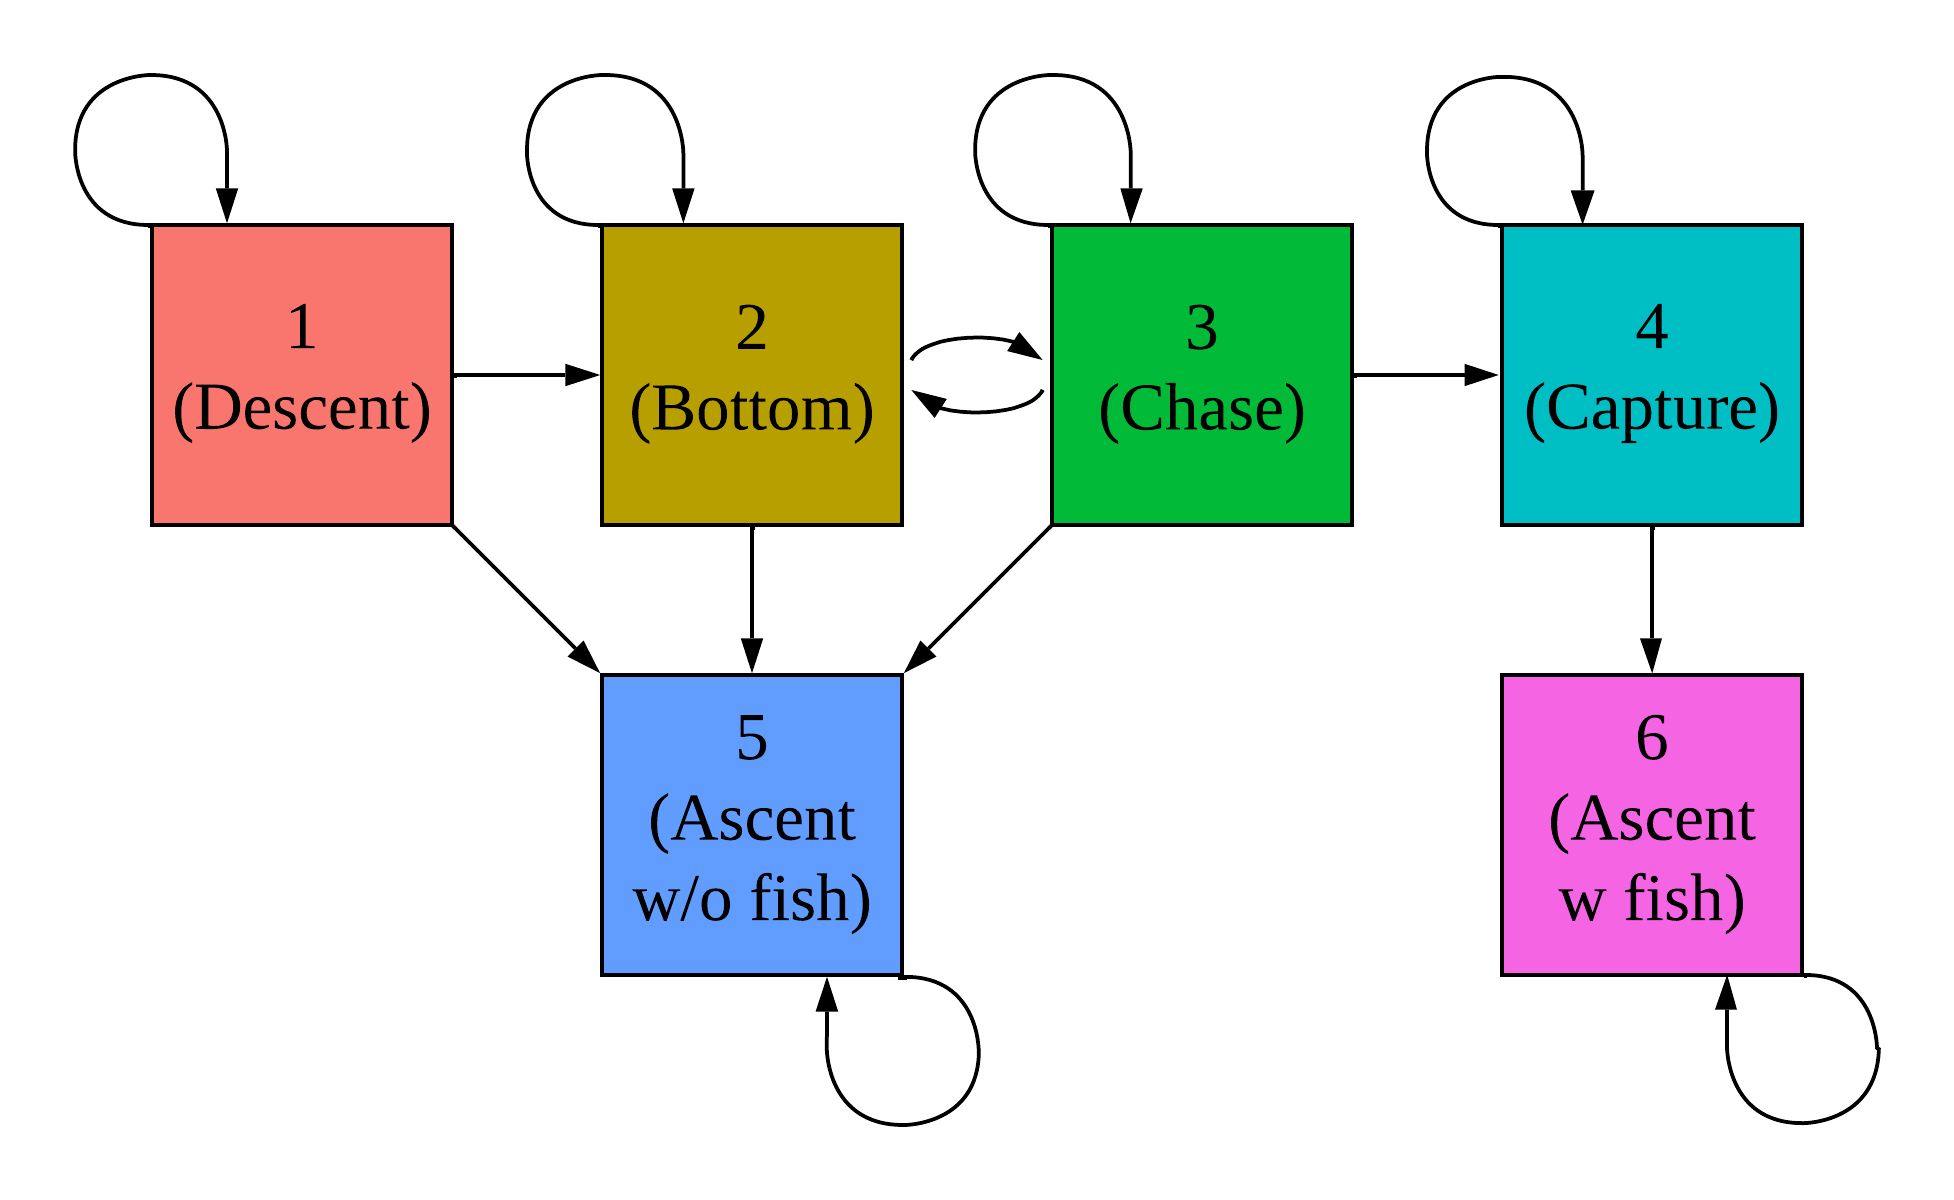
\includegraphics[width = 4in]{plt/PHMM_cs2.png}
    \caption{Visualization showing how the Markov chain $\bfX_s$ can evolve within the second case study of killer whale foraging. Arrows correspond to non-zero entries in $\bfGamma$, where arrows point from row number to column number. Within a dive, a killer whale can proceed from descent, to bottom, to chase, to capture, to ascent with fish. It can also ascend without a fish at any time before capture, and it can switch between the bottom and chase states freely.}
    \label{fig:PHMM_cs2}
\end{figure}

%The Markov chain defined in Figure \ref{fig:PHMM_cs2} shows possible subdive states for each two-second window, but I also want to decode successful foraging on a dive level. Luckily, denoting the number of windows within dive $s$ as $T_s$, the probability that dive $s$ contains successful foraging is simply $\bbP(X_{s,T_s} \in \{4,6\} \mid \bfY_s = \bfy_s)$ for all dives $s = 1,\ldots,130$.

Given that $X_{s,t} = i$, I modelled change in depth with a normal distribution, heading total variation with a gamma distribution, and normalized jerk peak with a gamma distribution. To enforce that the killer whale does not ascend or descend on average during the bottom of its dive, I set the state-dependent distributions of change in depth for the bottom, chase, and capture states to have a mean of zero. Further, I wanted to ensure that the model distinguished foraging based primarily on the ``prey capture" subdive state rather than differences between the ``ascent with a fish" and ``ascent without a fish" states. As such, I set the two state-dependent distributions associated with ascent to be identical. Given the hidden state of a window ($X_{s,t}$), I also assumed that all summary statistics %($D_{s,t}, H_{s,t}$, and $J_{s,t}$) 
were independent. Denote the observations from dive $s$ as $\bfy_s = \{y_{s,t}\}_{t=1}^{T_s}$ and the labels from dive $s$ as $\bfz_s = \{z_{s,t}\}_{t=1}^{T_s}$. Then, I modelled all dives as independent, so the total likelihood for the model with weighting parameter $\alpha$ and parameters $\bfdelta, \bfGamma, \bftheta$ and $\bfbeta$ was $\prod_{s=1}^{130} p_\alpha (\bfy_s,\bfz_s ~;~ \bfdelta, \bfGamma, \bftheta,\bfbeta)$, where $p_\alpha$ is defined in Equation (\ref{eqn:PHMM_like_alpha}). 

\subsubsection{Model Evaluation}

I fit five different PHMMs corresponding to $\alpha \in \{0.0001,0.001,0.01,0.1,1\}$. I did not include $\alpha = 0$ in this case study because I did not have labels associated with subdive states 2 and 3 (bottom and chase). Thus, if $\alpha = 0$, there were no observations that could be used to estimate the parameters of the state-dependent distribution parameters $\theta^{(2)}$ and $\theta^{(3)}$, and the model would not be identifiable. 

In addition to the PHMMs, I also implemented the prey-capture identification method from \citet{Tennessen:2019a} as a baseline. In particular, \citet{Tennessen:2019a} calculated three summary statistics for each dive: (1) the maximum of jerk during the bottom 70\% of the dive, divided by the median jerk during the same period, (2) the absolute value of the killer whale's roll at the moment of jerk peak, and (3) the circular variance of heading during the bottom 70\% of the dive. Then, \citet{Tennessen:2019a} took the minimum value of every summary statistic over all confirmed prey capture dives to obtain thresholds for each of the three dive-level summary statistics. Finally, a dive was labelled as a successful foraging dive if \textit{every} dive-level summary statistic surpassed that threshold.

I evaluated each model based on how well it predicted successful foraging dives. Note that the probability that dive $s$ is a successful foraging dive is equal to the probability that it ends in either the capture or ascent with fish state. In other words, it is the probability that window $T_s$ of dive $s$ has subdive state 4 (capture) or subdive state 6 (ascent with fish), or $\bbP(X_{s,T_s} \in \{4,6\} \mid \bfY_s = \bfy_s)$. To estimate this value, I randomly and equally split the seven labelled successful foraging dives and 19 labelled dives without successful foraging into four folds and performed cross validation with the forward-backward algorithm. I calculated AUC values within each fold and reported their averages (see Figure \ref{fig:AUCs_cs2}). Finally, I also fit each PHMM to the entire dataset to visualize their state-dependent distributions (see Figure \ref{fig:emissions}). 

\subsubsection{Results}

My method outperformed the baseline of \cite{Tennessen:2019a}, which had an average AUC of $0.79$. In comparison, the PHMM with $\alpha = 0.0001$ had an average AUC of $0.90$, the PHMM with $\alpha = 1.0$ had an AUC of $0.96$, and the PHMM with $\alpha = 0.01$ had a perfect AUC of $1$ across all four folds (Figure \ref{fig:AUCs_cs2}). Thus, not only did using a PHMM produce better predictive performance over existing baselines, but using $\alpha \in (0,1)$ (namely $\alpha = 0.01$ here) improved predictive performance over $\alpha = 0$ and $\alpha = 1$.

\begin{figure}
    \centering
    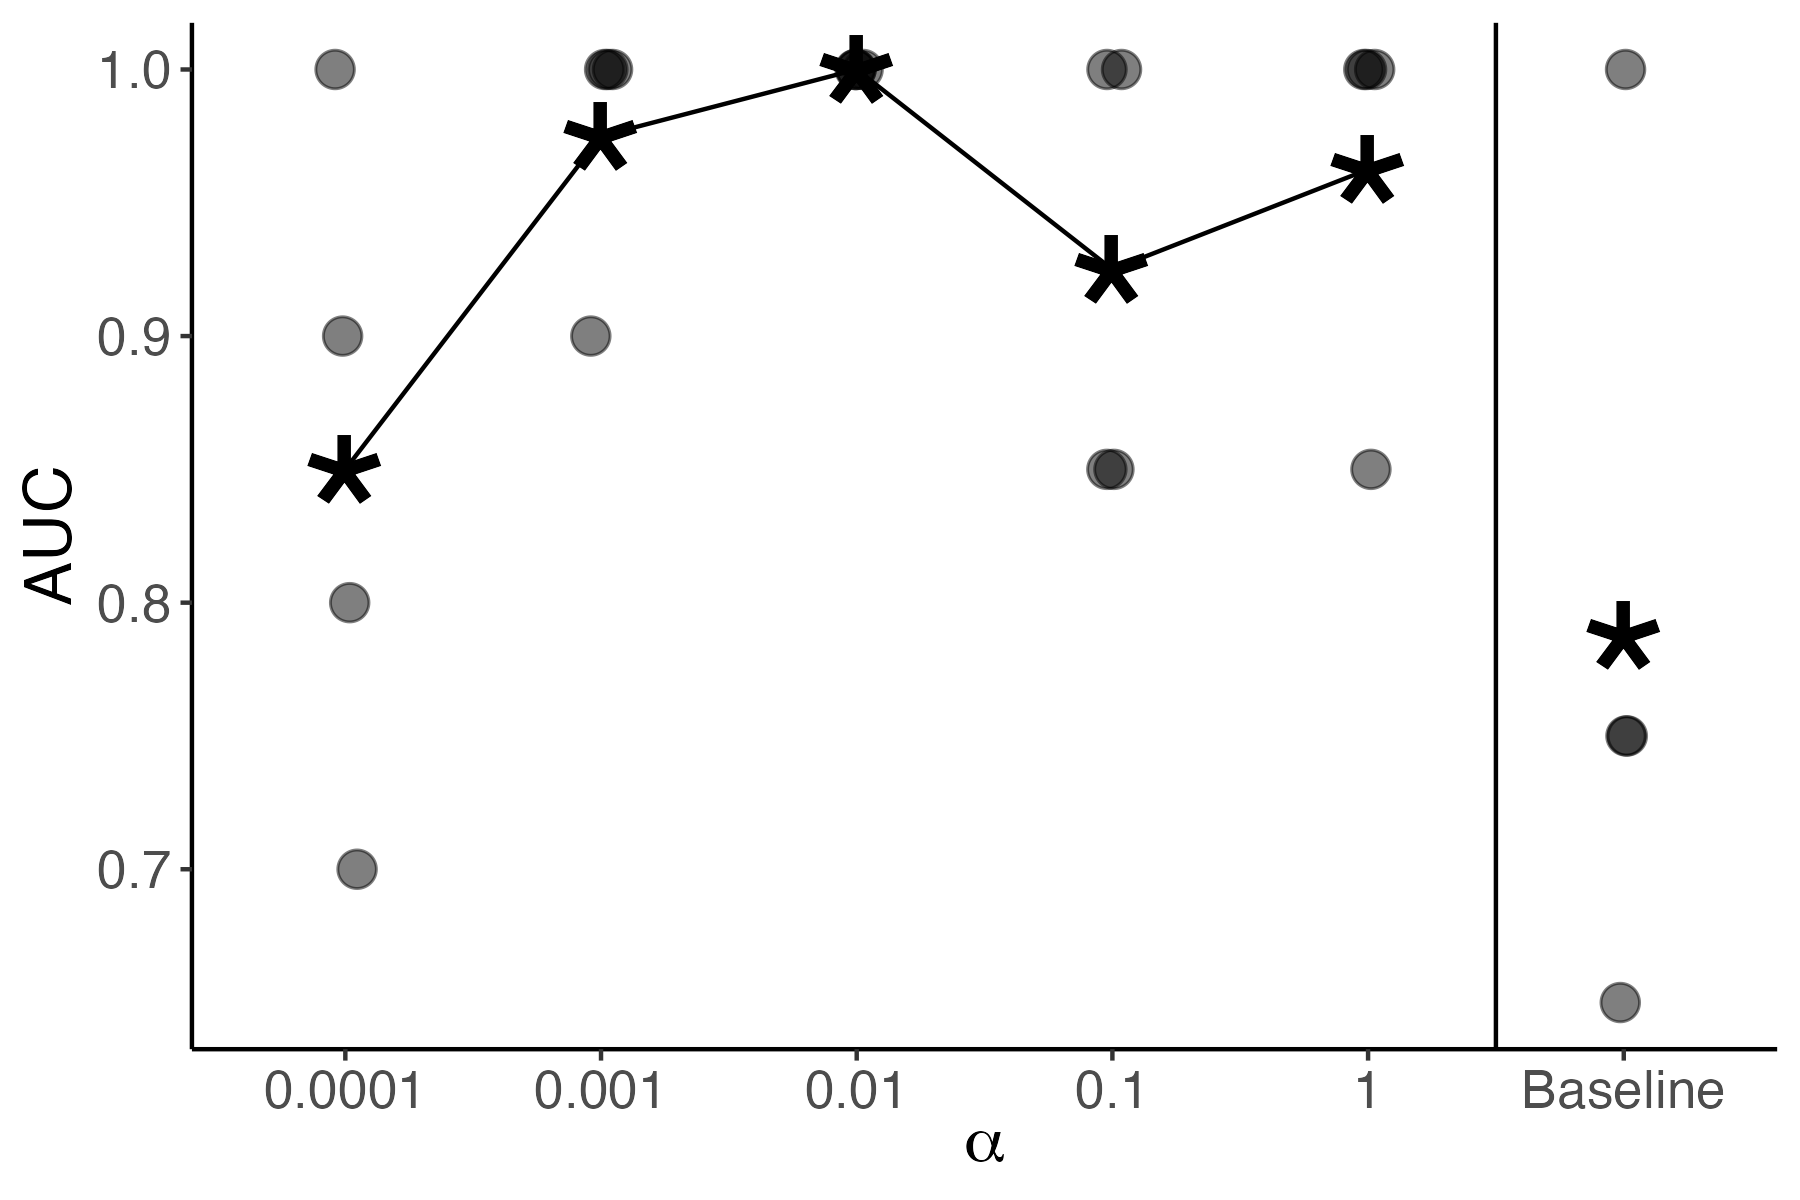
\includegraphics[width = 4in]{plt/AUCs_delt_d_htv_jp_normed_4.png}
    \caption{Four-fold, cross-validated area under the ROC curve (AUC) values for five PHMMs as well as the baseline method of \citet{Tennessen:2019a}. Horizontal jitters have been added because dots occasionally fall on top of one another. Averages are shown as stars and connected with a line for the PHMM approaches.}
    \label{fig:AUCs_cs2}
\end{figure}

The biological interpretation of each PHMM heavily depended on the weight $\alpha$. For example, the ``bottom" and ``chase" states looked very similar for the PHMMs with $\alpha \leq 0.01$, but the two states were better separated within the PHMM with $\alpha = 1$ (Figure \ref{fig:emissions}). %This implies that setting $\alpha$ much lower than 1 may result in a slightly less biologically interpretable model. However, the PHMM with $\alpha = 0.01$ had better predictive performance than the PHMM with $\alpha = 1$, so practitioners may have to balance these two considerations when deciding on an optimal weight $\alpha$. 
However, the ``bottom" subdive state had higher mean jerk peak and heading total variation than the ``chase" subdive state for the PHMM with $\alpha = 1$. These results are the opposite of what ecologists expect biologically, indicating that a large separation between state-dependent distributions is not always more biologically interpretable. I conjecture that the ``bottom" and ``chase" subdive states are particularly unintuitive partially because there are no labels associated with either of these subdive states (i.e. $z_{s,t} \neq 2,3$ for any $s$ or $t$). As a result, there is little information for the model to differentiate the two subdive states. 

\begin{figure}
    \centering
    \begin{subfigure}[t]{0.45\textwidth}
        \centering
        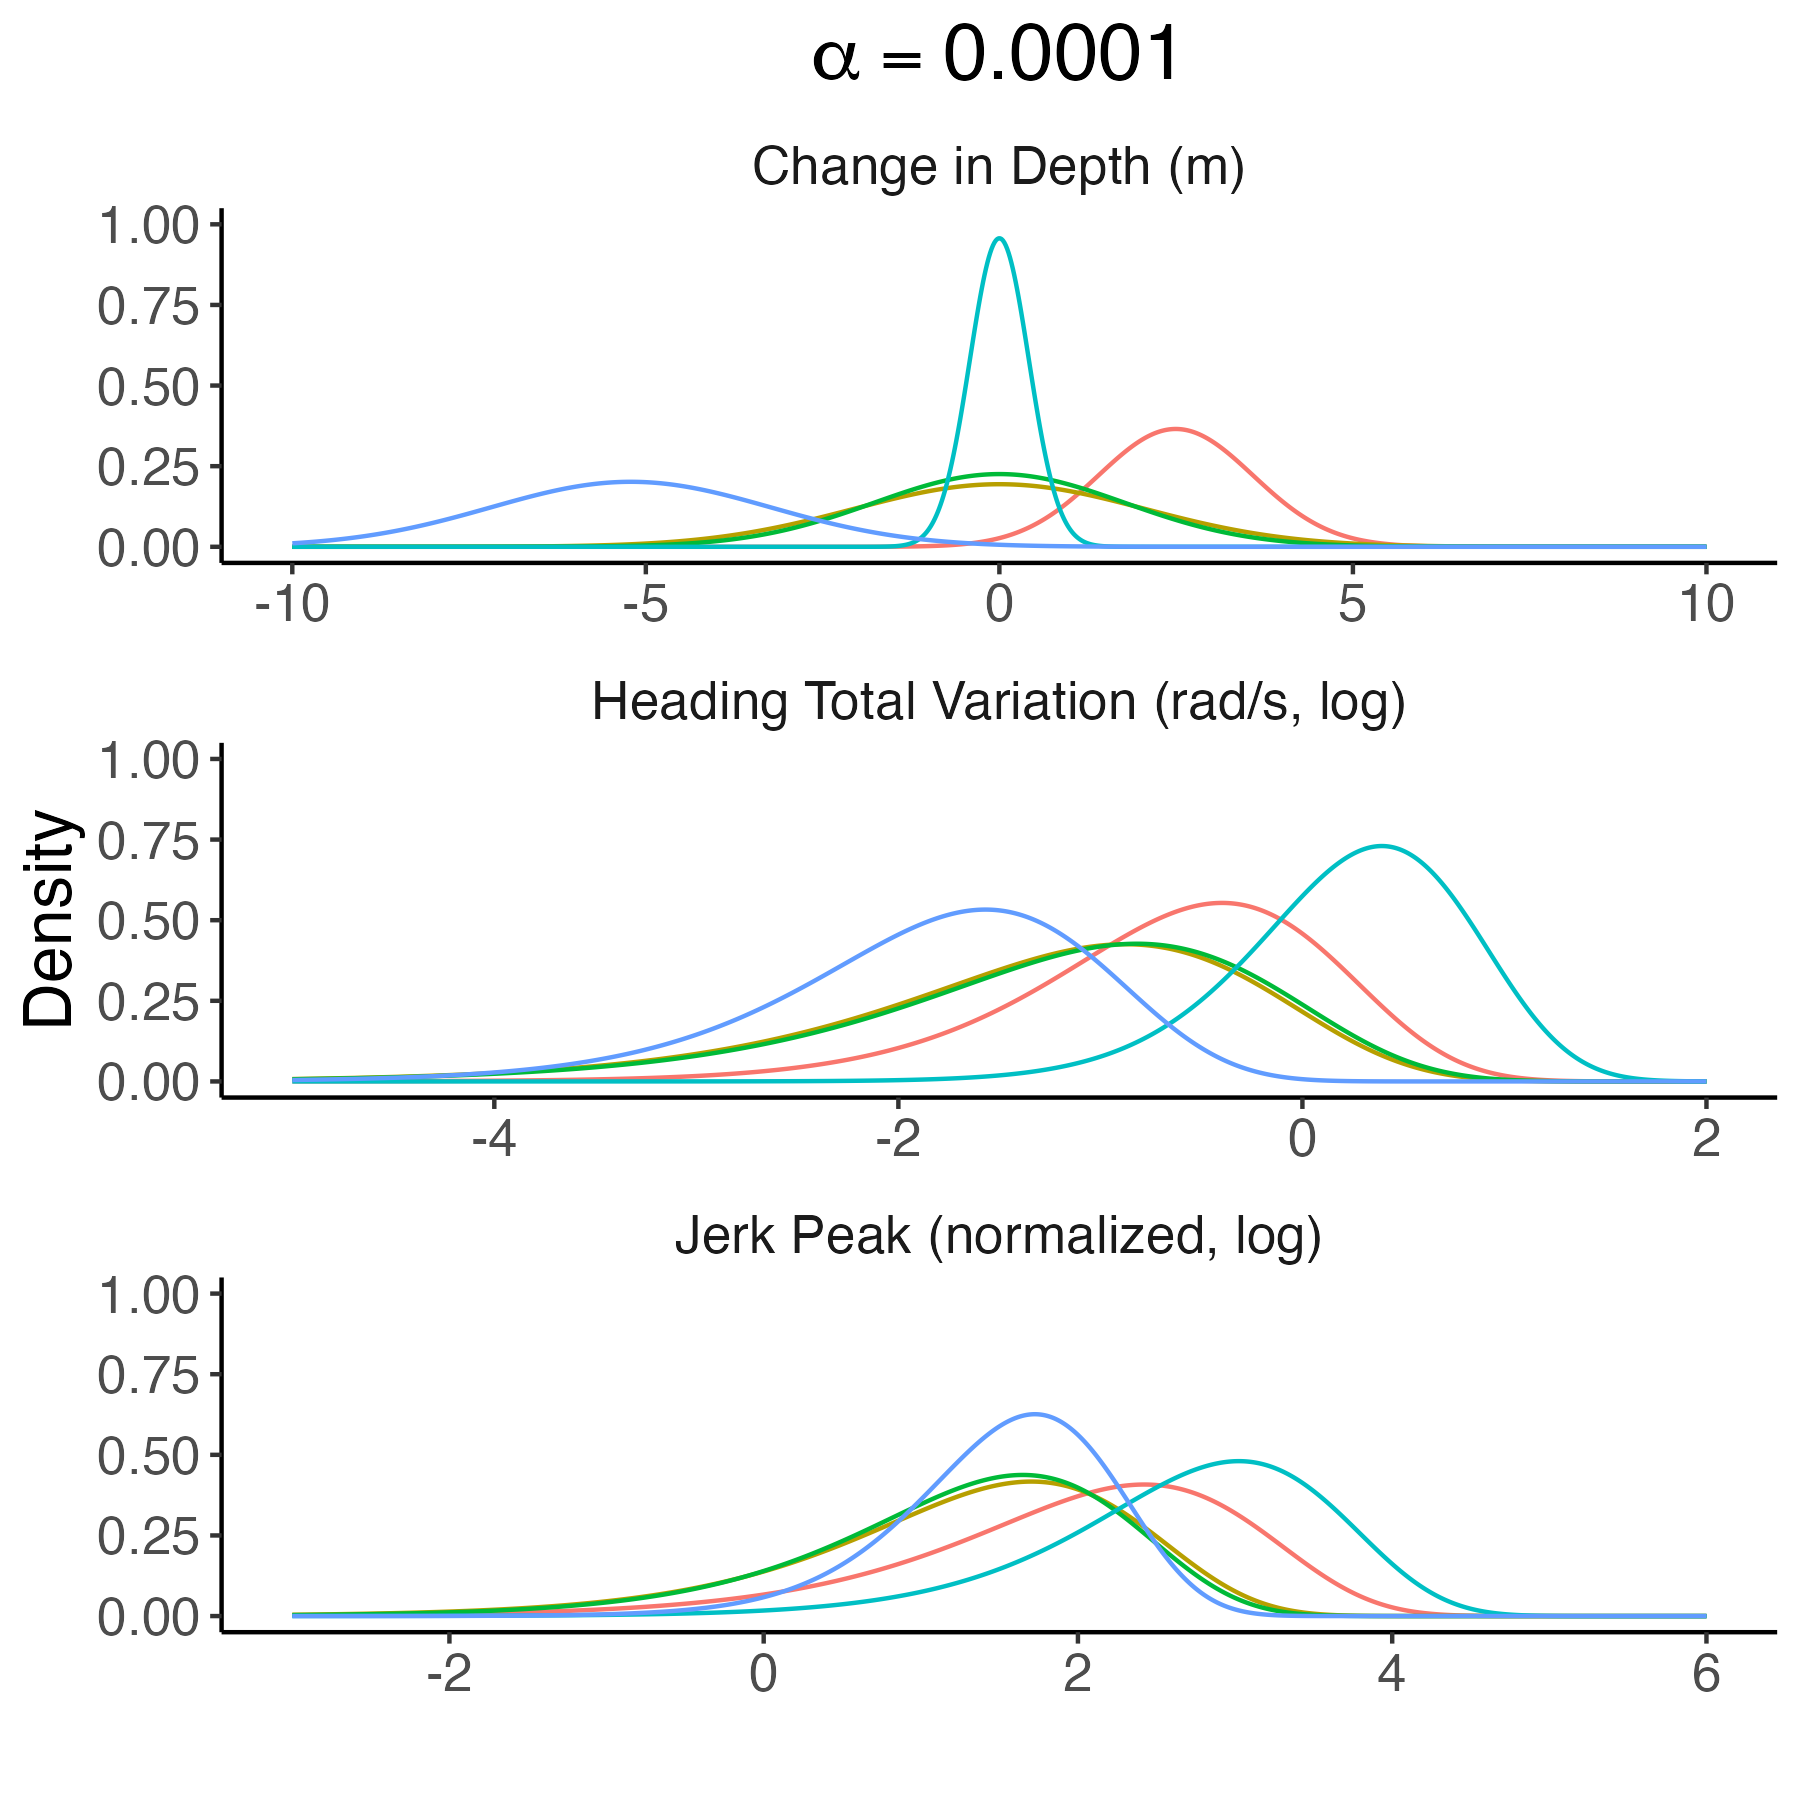
\includegraphics[height = 2.75in]{plt/emissions_delt_d_htv_jp_normed_-4_1.png}
        \caption{$\alpha = 0.0001$}
    \end{subfigure}
    ~
    \begin{subfigure}[t]{0.45\textwidth}
        \centering
        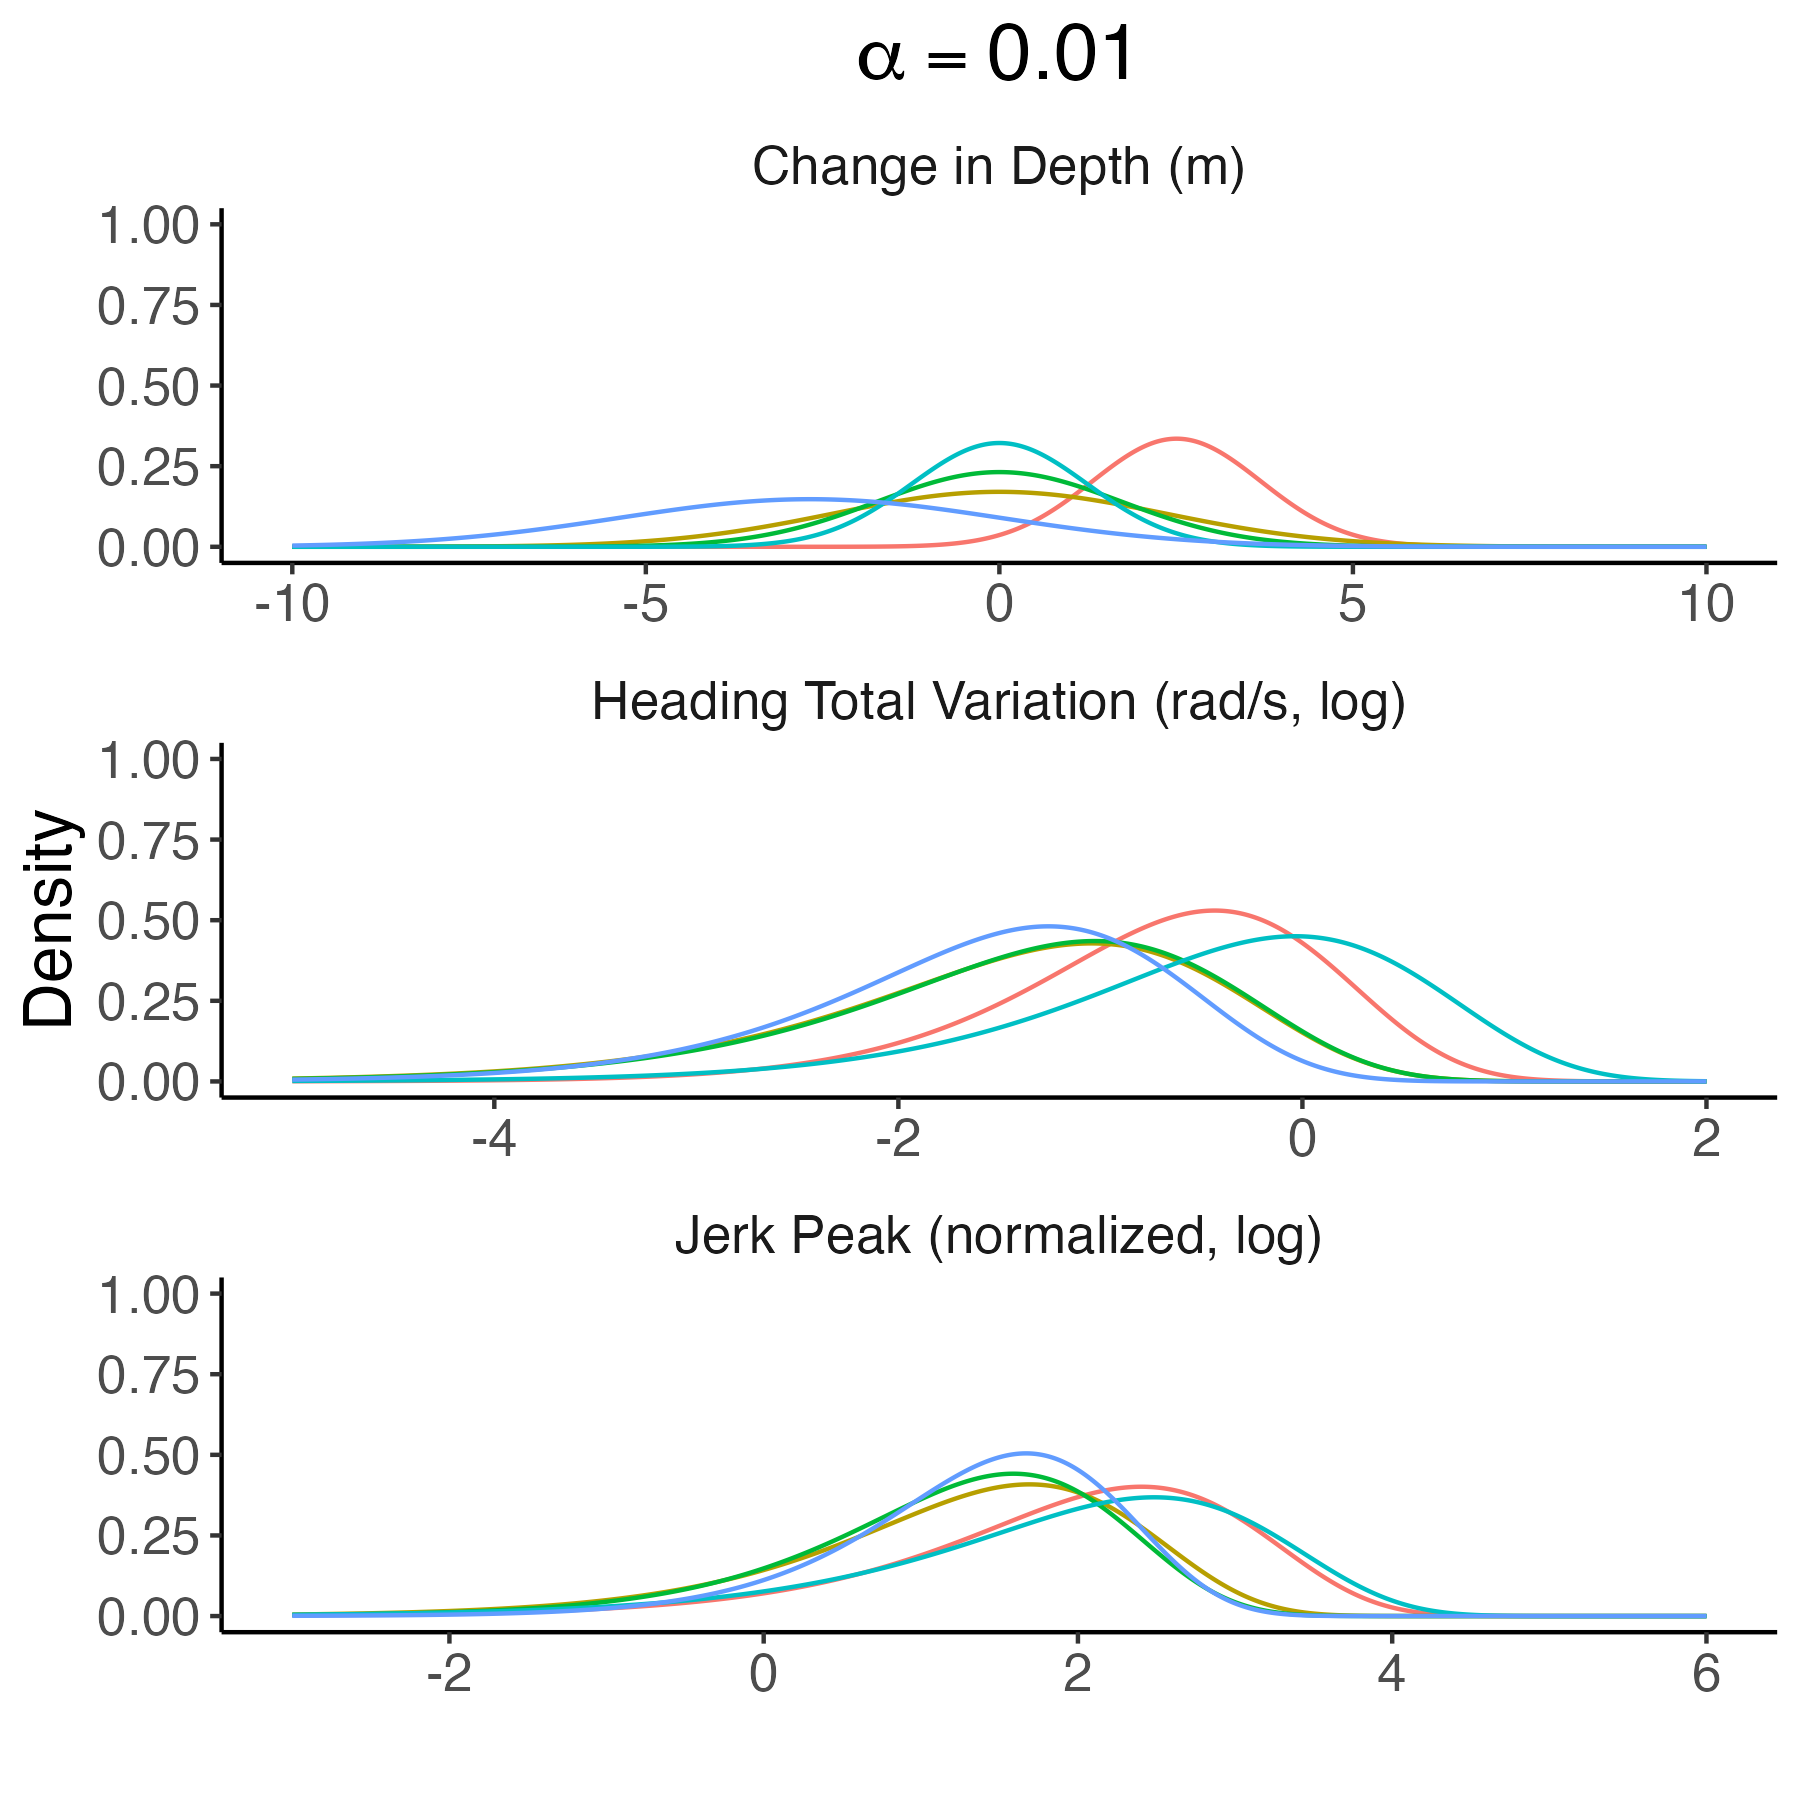
\includegraphics[height = 2.75in]{plt/emissions_delt_d_htv_jp_normed_-2_1.png}
        \caption{$\alpha = 0.01$}
    \end{subfigure}
    \\
    \begin{subfigure}[t]{0.9\textwidth}
        \centering
        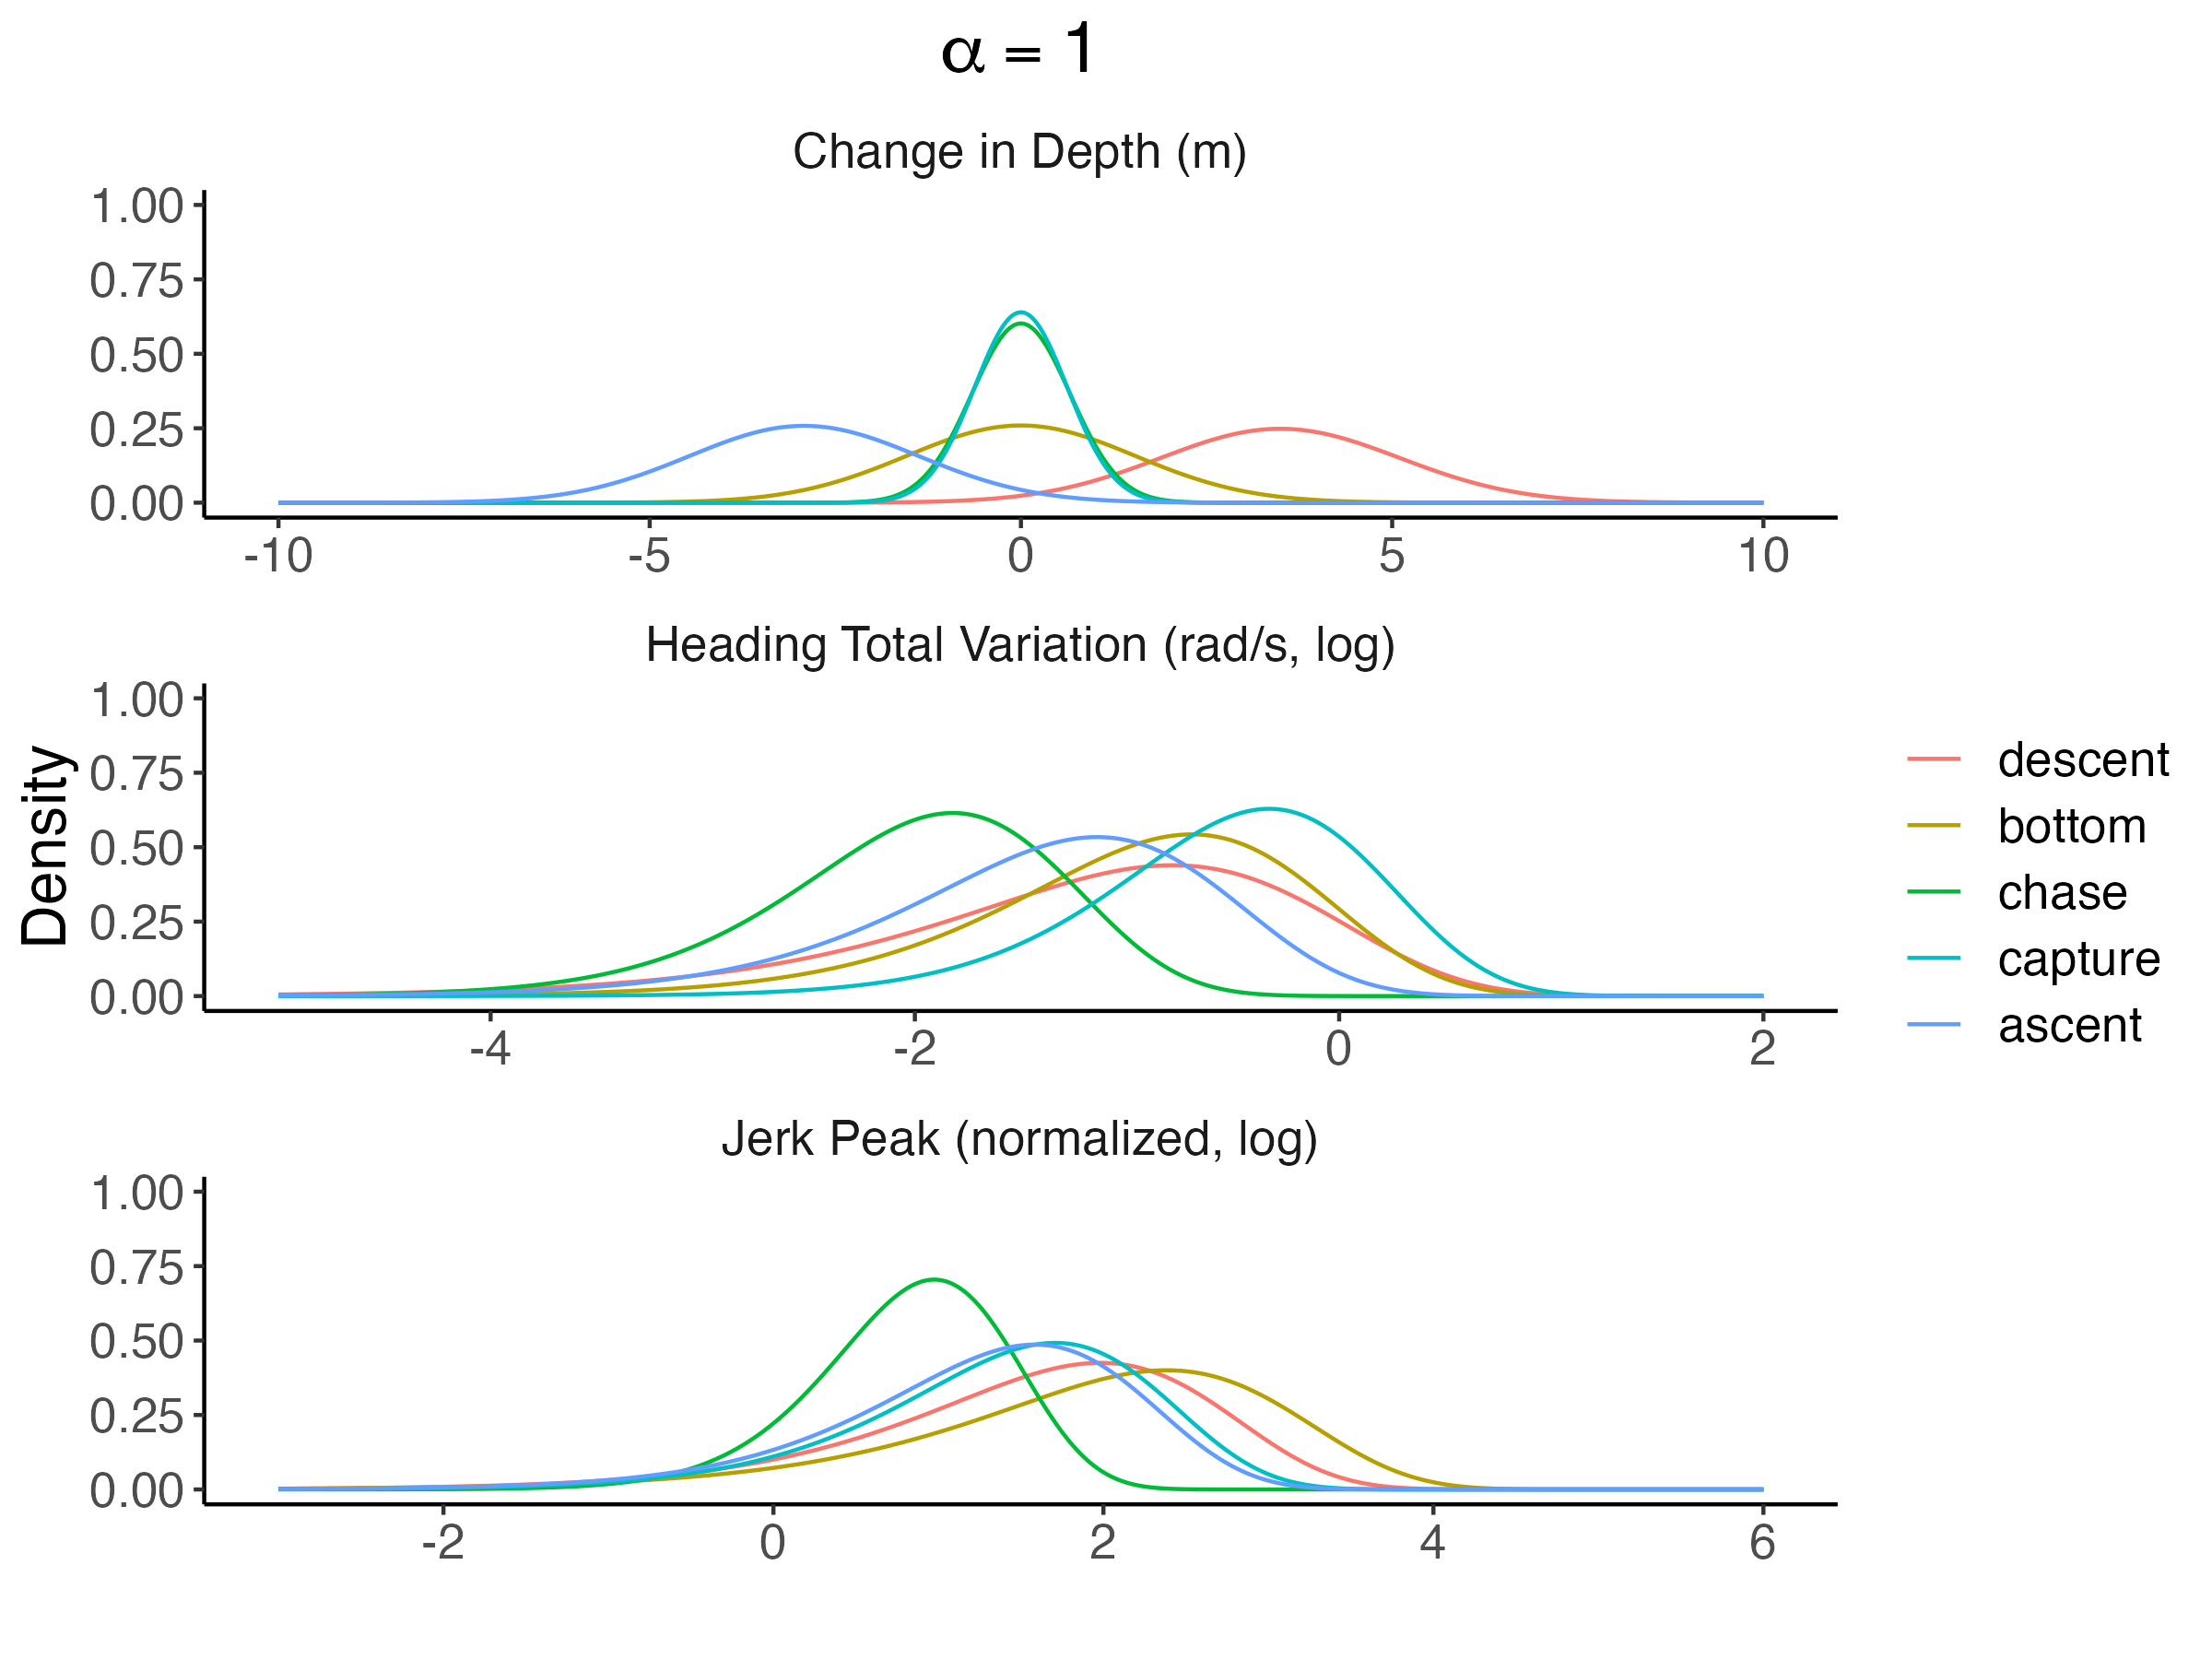
\includegraphics[height = 2.75in]{plt/emissions_delt_d_htv_jp_normed_0_1.png}
        \caption{$\alpha = 1$}
    \end{subfigure}
    \caption{State-dependent densities for change in depth (top panels), heading total variation (middle panels), and normalized jerk peak (bottom panels) for PHMMs with $\alpha = 0.0001$ (top left), $\alpha = 0.01$ (top right), and $\alpha = 1$ (bottom). Densities are coloured according to their corresponding subdive state. Parameters were estimated using the entire killer whale dataset (i.e. no cross-validation was performed). For a given observation $Y_{s,t}$, all features were assumed to be independent after conditioning on the subdive state $X_{s,t}$. Note that the ``ascent with a fish" and ``ascent without a fish" states were assumed to have identical distributions, so both are listed simply as ``ascent".}
    \label{fig:emissions}
\end{figure}

%As $\alpha$ increased, the estimated mean of jerk peak and estimated mean of heading total variation associated with the capture state decreased. Likewise, the estimated standard deviation associated with the capture state for all three features increased as $\alpha$ increased from 0 to 0.01, and then decreased again as $\alpha$ increased from 0.01 to 1 (Figure \ref{fig:emissions}).

Differences between each model's distribution for the capture state appeared to impact predictive performance. 
%
For example, the PHMM with $\alpha = 0.0001$ estimated a relatively high mean and low standard deviation for heading total variation (middle panel of Figure \ref{fig:emissions}a). As such, it failed to identify a prey capture event in which heading total variance was highly variable (Figure \ref{fig:profiles_5975}).
%
Alternatively, the PHMM with $\alpha = 1$ estimated a relatively low mean for heading variation (middle panel of Figure \ref{fig:emissions}c). As a result, it was often too sensitive and decoded some dives that lacked successful foraging as containing a prey capture state (Figure \ref{fig:profiles_5489}). 
%
The PHMM with $\alpha = 0.01$ estimated a high mean and a high standard deviation for heading total variation (middle panel of Figure \ref{fig:emissions}b). It correctly identified a wide variety of labelled foraging dives, but it was not overly sensitive and correctly identified low-activity dives as lacking successful foraging.

\begin{figure}
    \centering
    \begin{subfigure}[t]{0.45\textwidth}
        \centering
        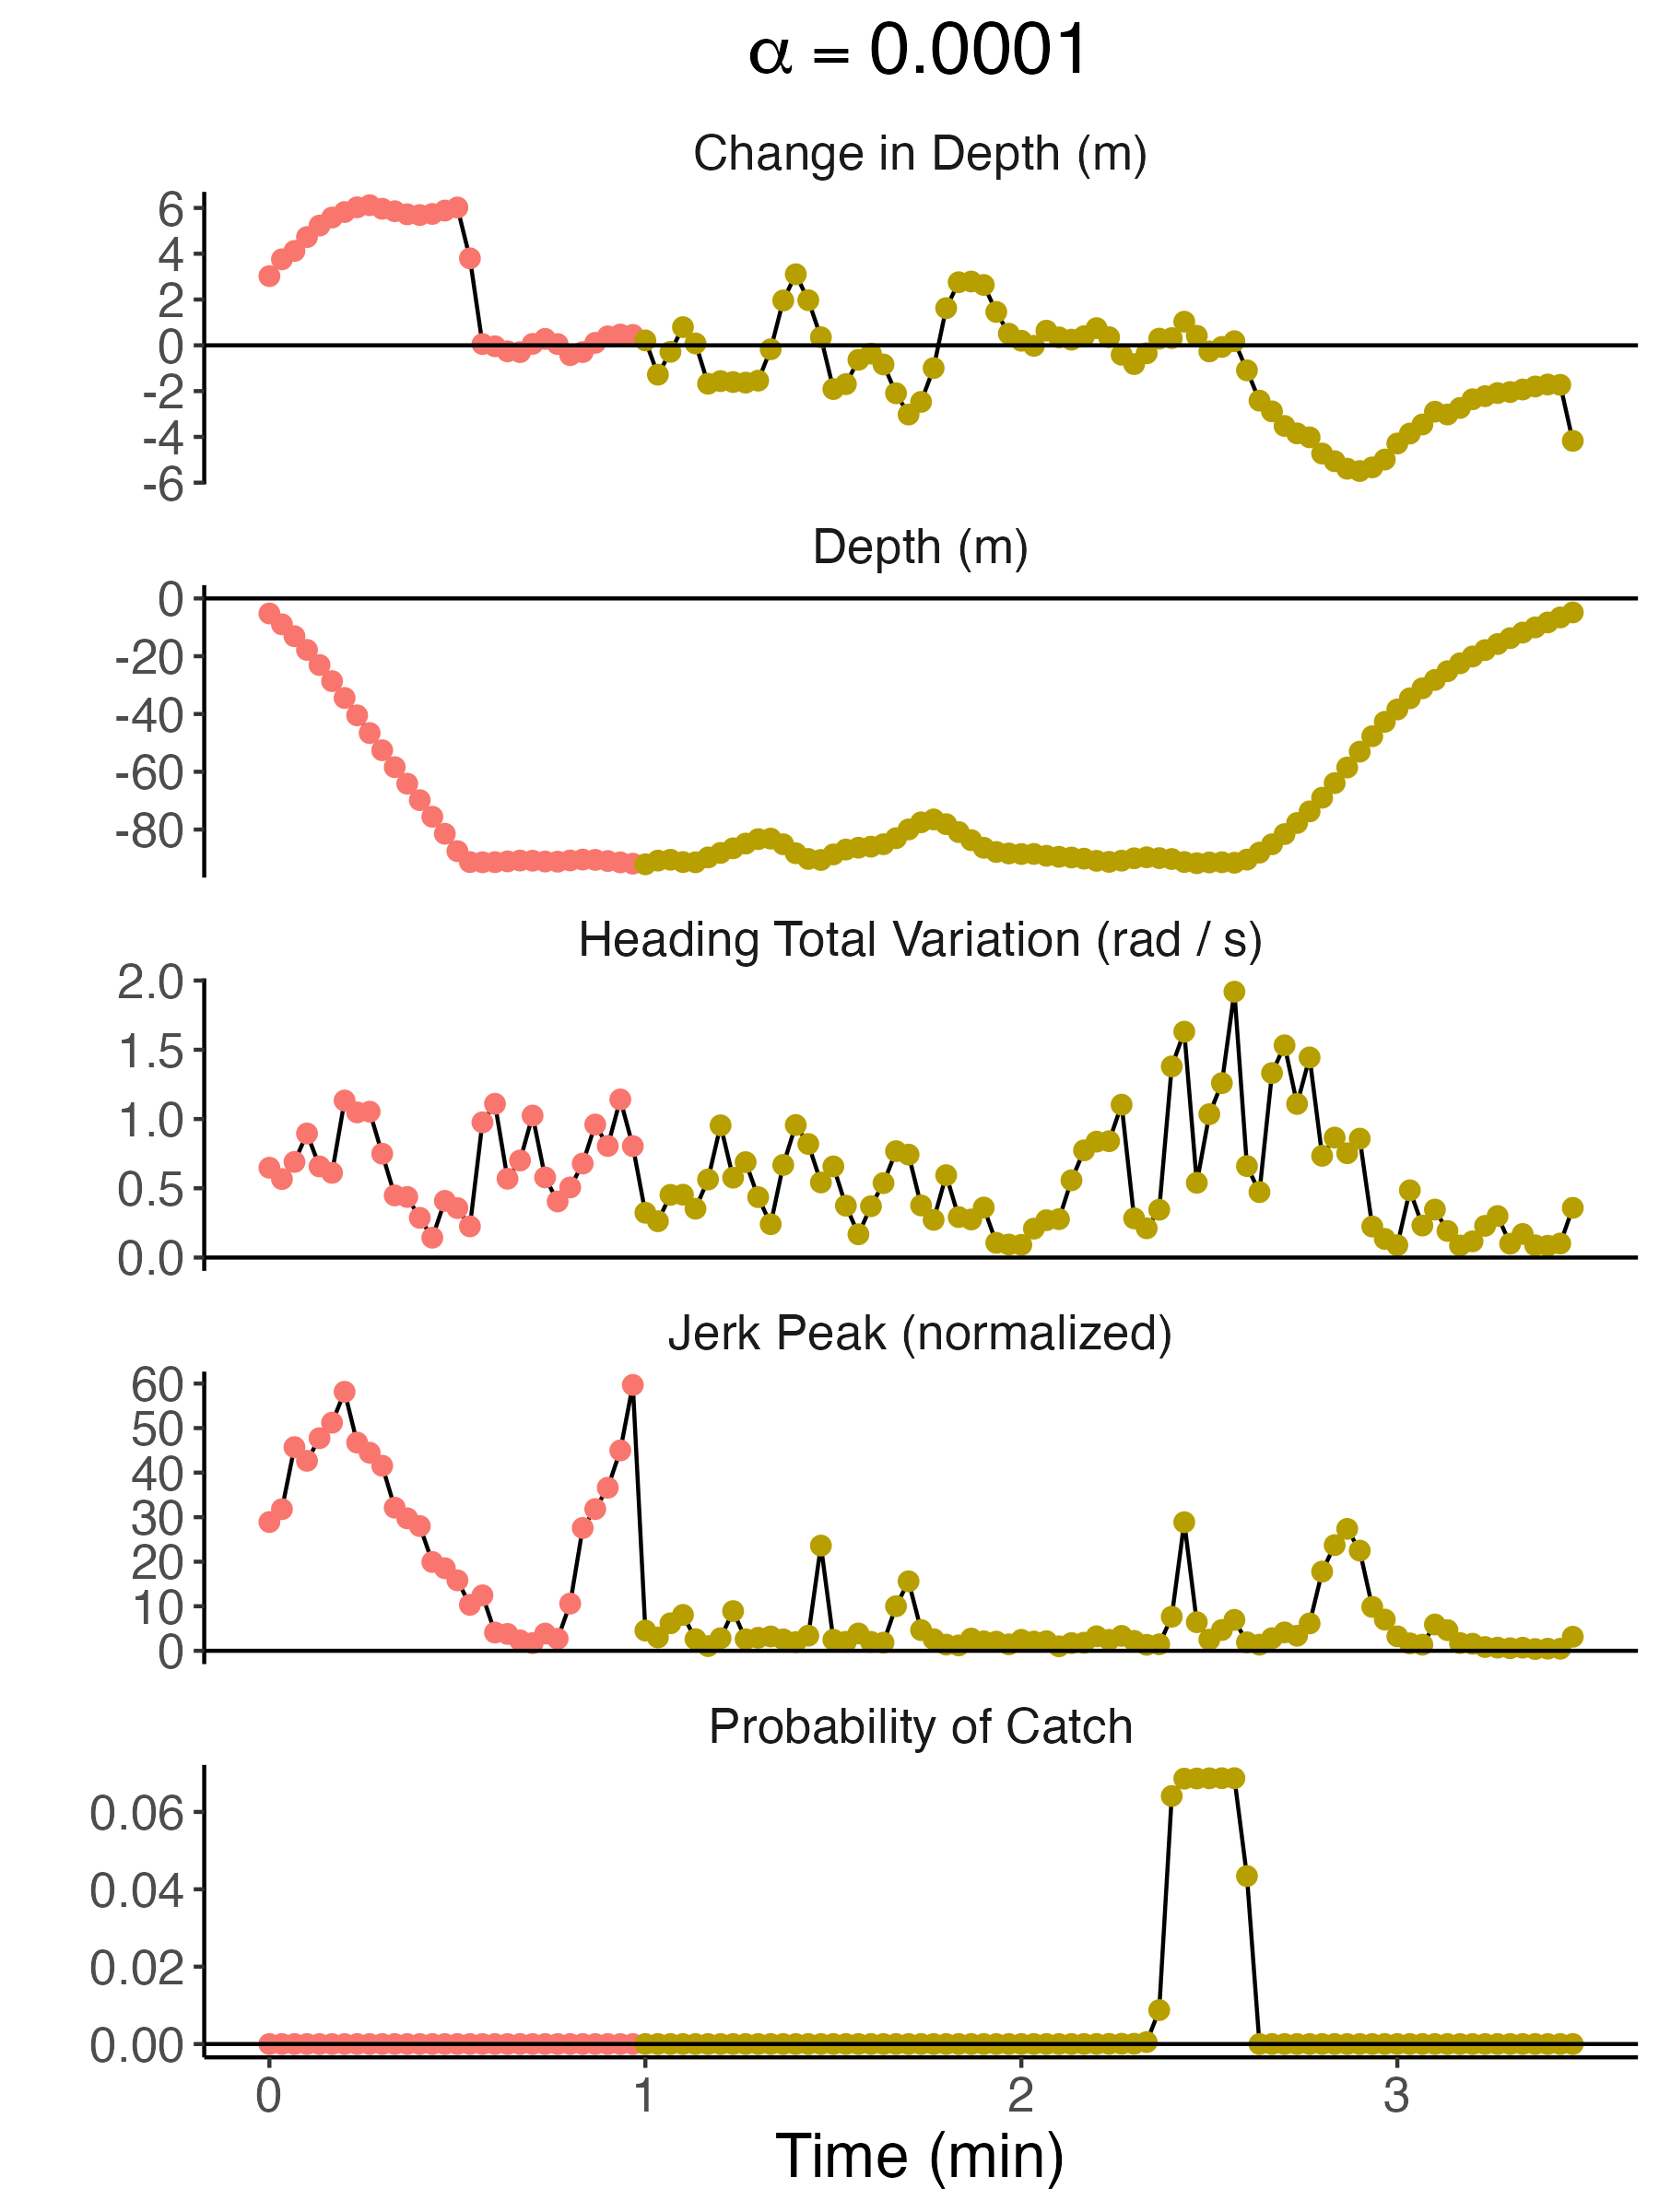
\includegraphics[height = 3.75in]{plt/profile_delt_d_htv_jp_normed_-4_4_pos_5975.png}
        %\caption{Decoded dives for PHMM with $\alpha = 0.0001$ (severely down-weighting unlabelled observations).}
    \end{subfigure}
    ~
    \begin{subfigure}[t]{0.45\textwidth}
        \centering
        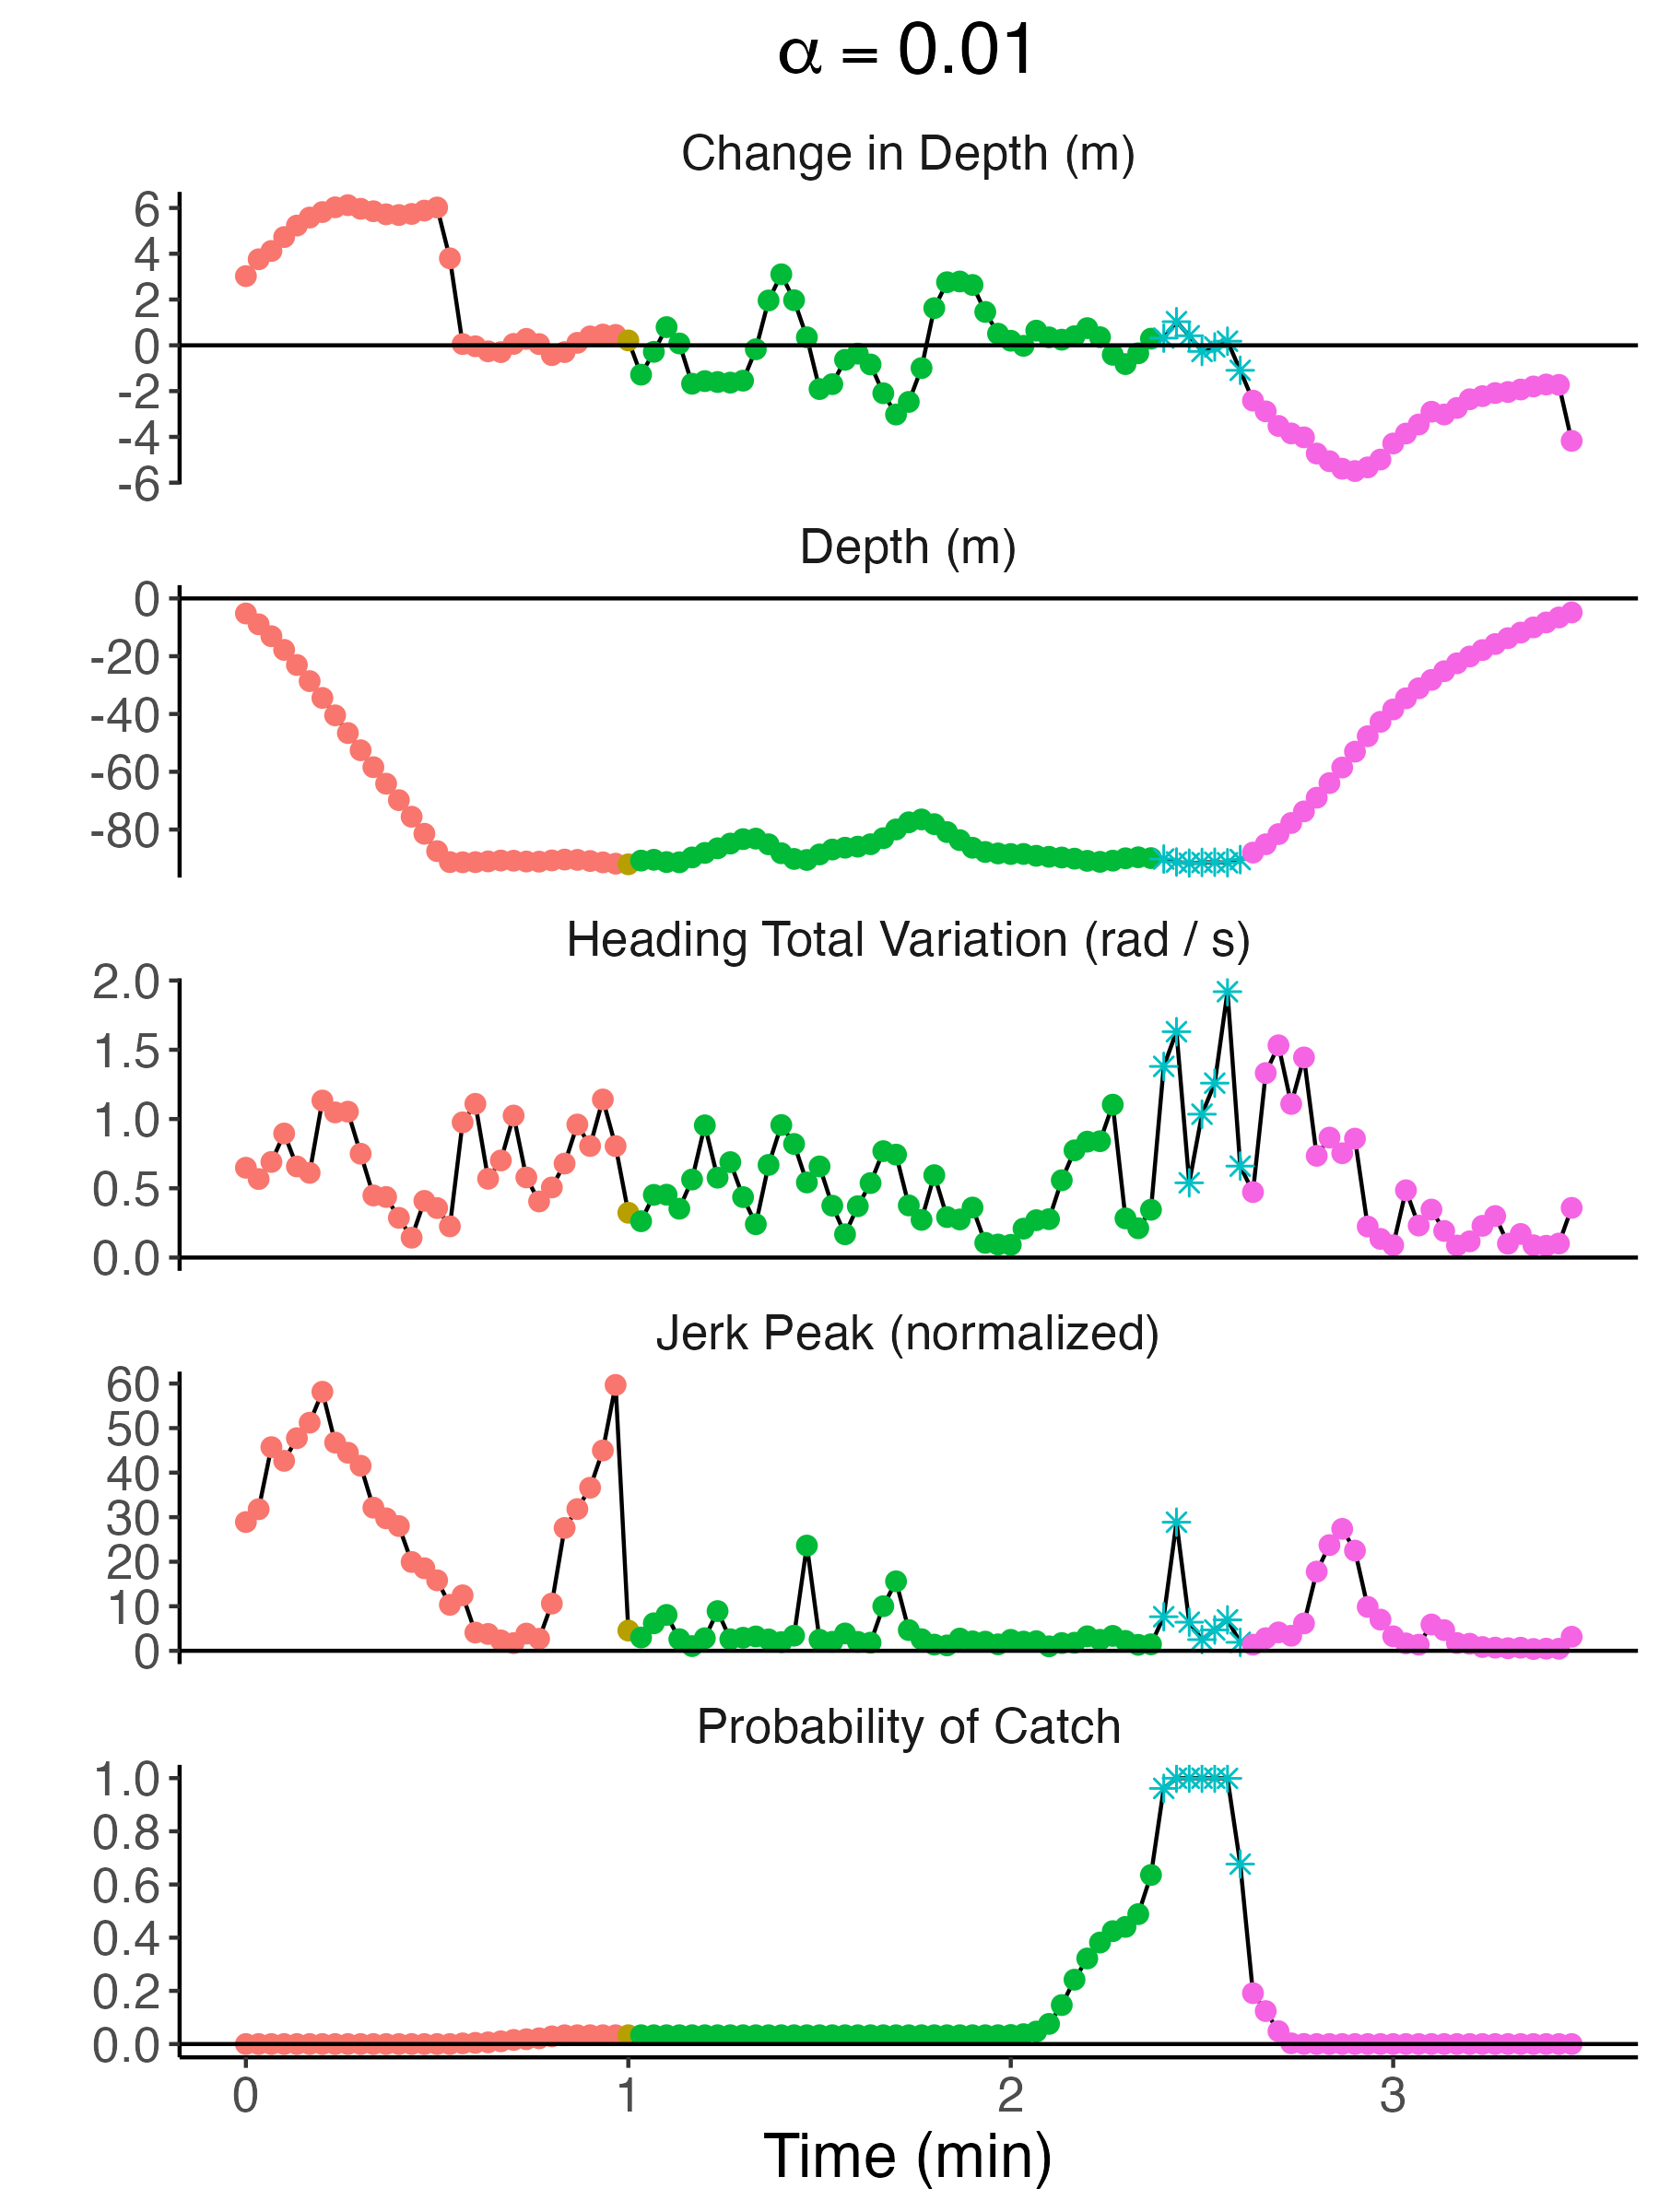
\includegraphics[height = 3.75in]{plt/profile_delt_d_htv_jp_normed_-2_4_pos_5975.png}
        %\caption{Decoded dive for PHMM with $\alpha = 0.01$ (down-weighting unlabelled observations).}
    \end{subfigure}
    \\
    \begin{subfigure}[t]{0.9\textwidth}
        \centering
        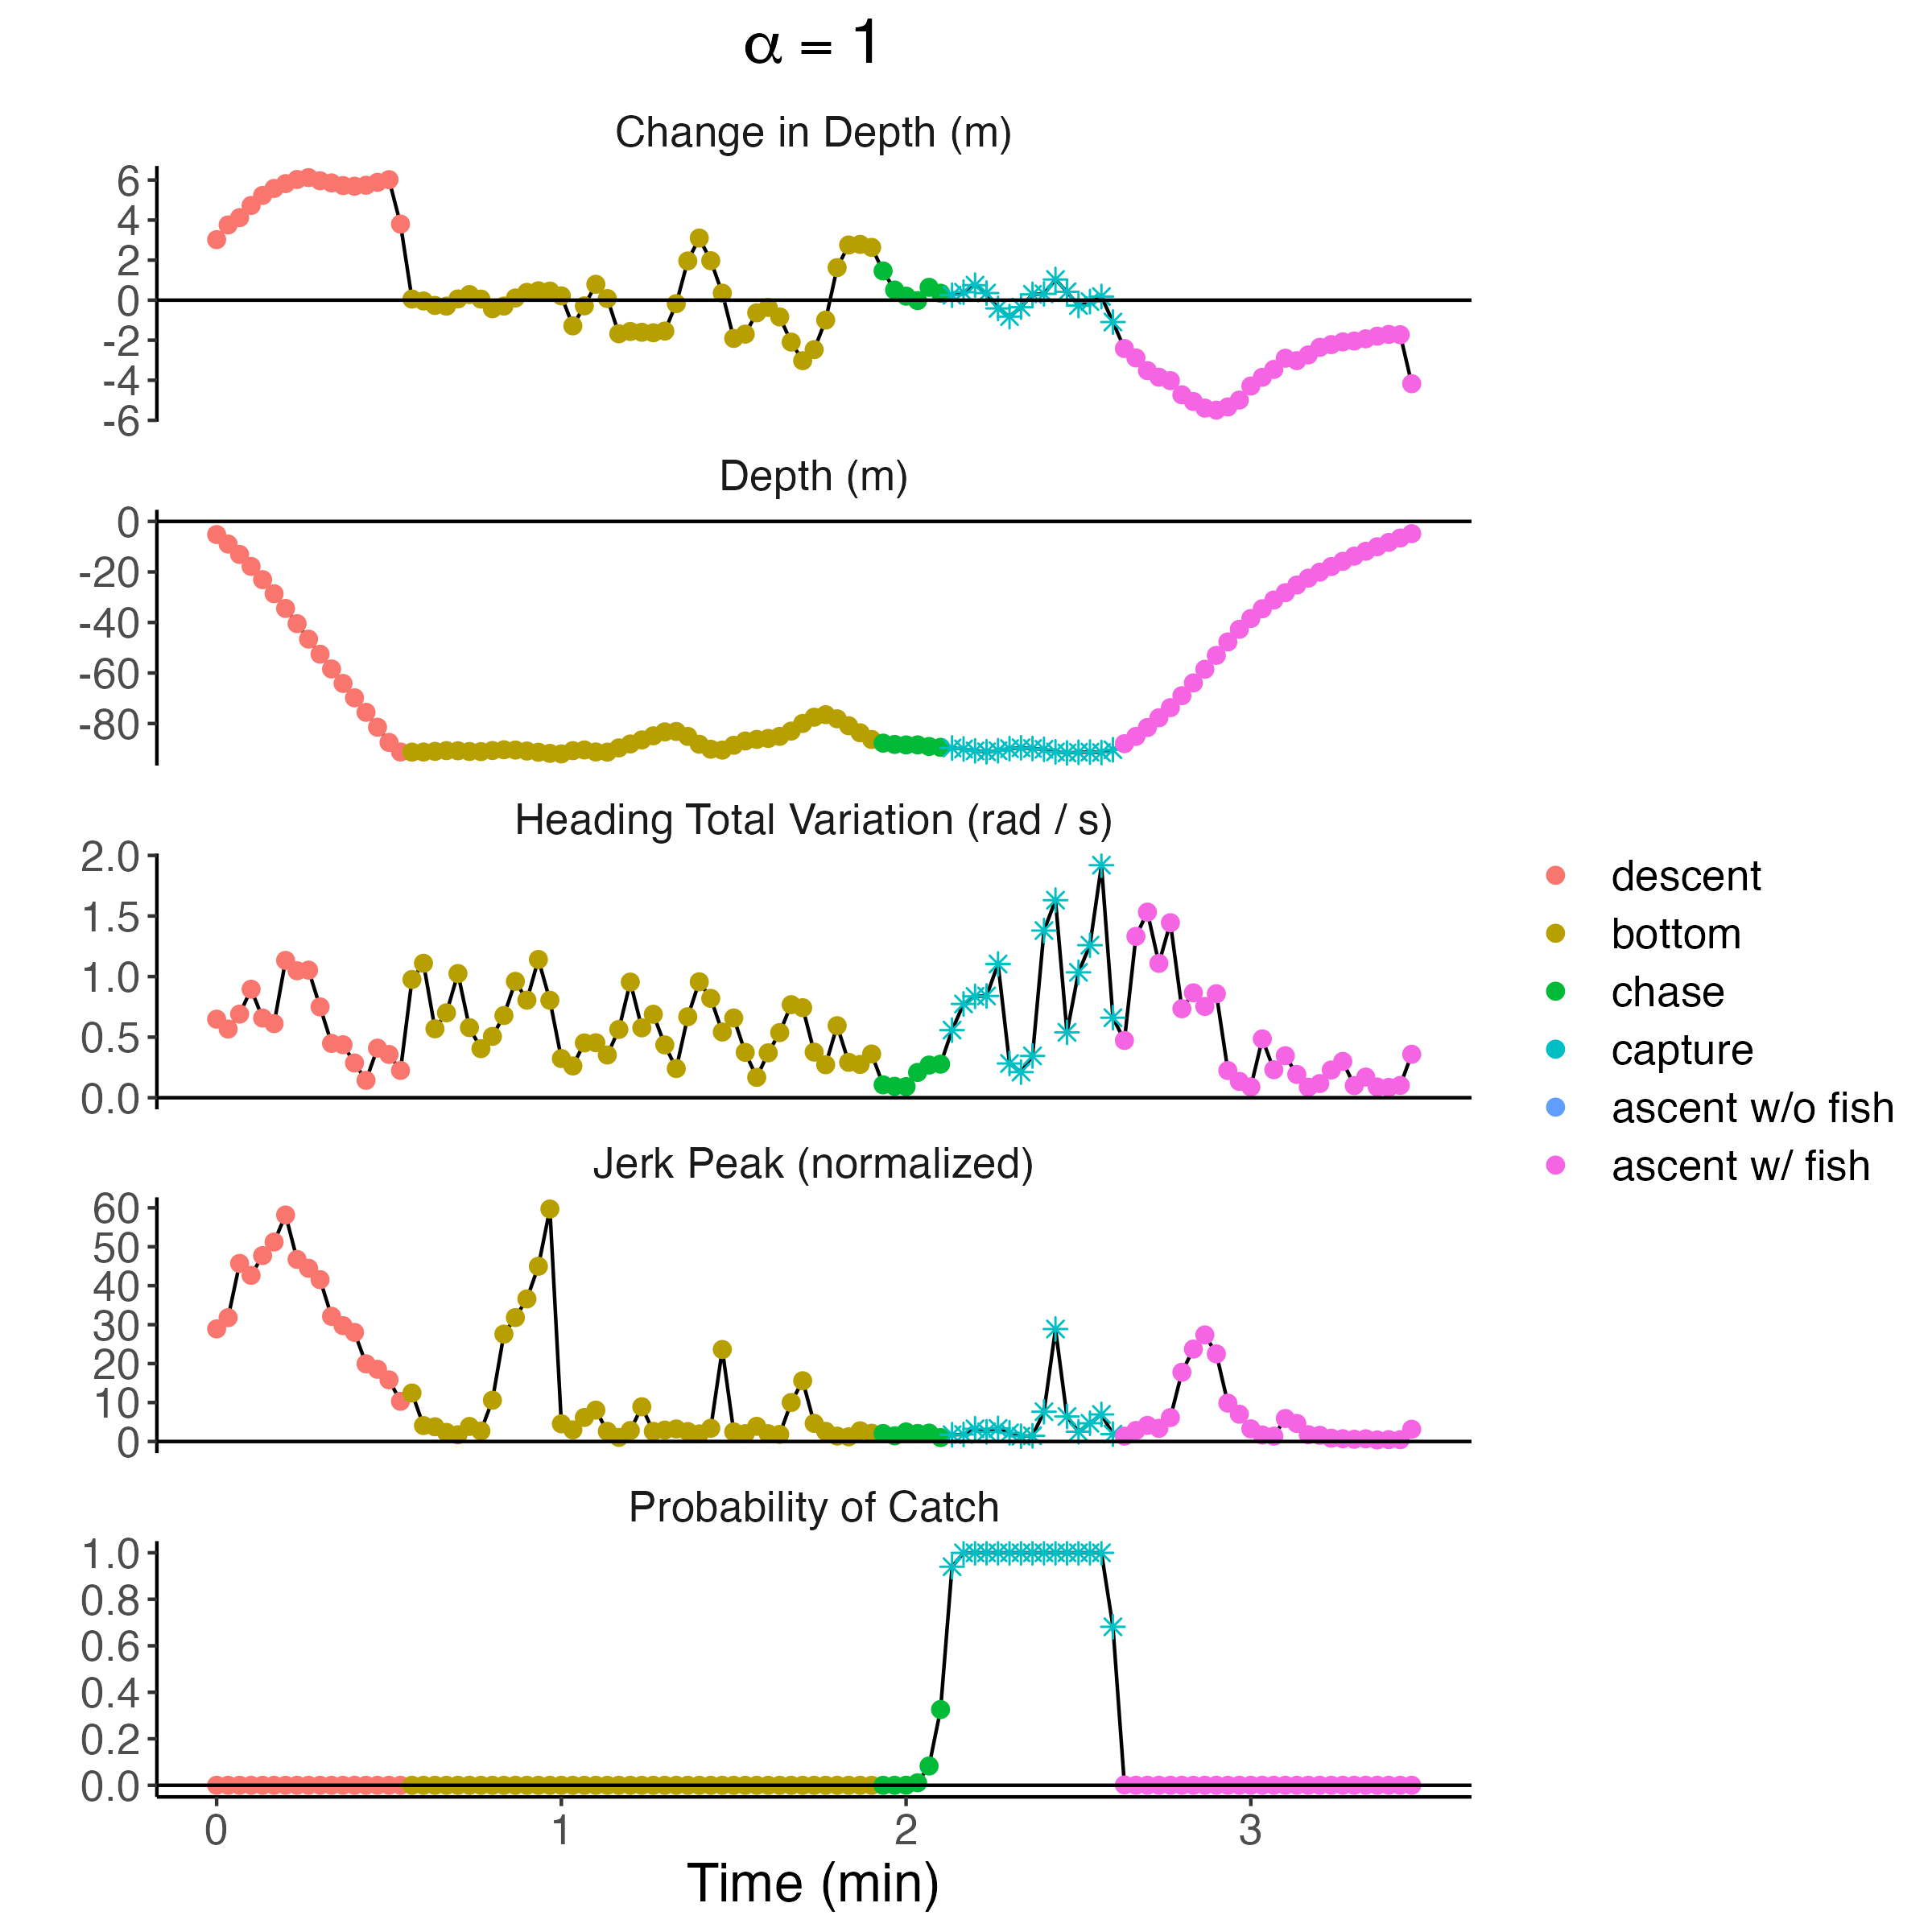
\includegraphics[height = 3.75in]{plt/profile_delt_d_htv_jp_normed_0_4_pos_5975.png}
        %\caption{Decoded dives for PHMM with $\alpha = 1$ (the ``natural" weighting).}
    \end{subfigure}
    \caption{Dive profiles, observations, and the decoded probability that each window is the ``capture" state for a selected successful foraging dive in case study 2. PHMMs with $\alpha = 0.0001$ (top left), $\alpha = 0.01$ (top right) and $\alpha = 1$ (bottom) are shown. Each subplot displays change in depth (top panel), raw depth (second panel), heading total variation (third panel), normalized jerk peak (fourth panel), and probability of ``capture" (bottom panel). Observations are coloured according to the most-likely sequence of hidden states as determined by the Viterbi algorithm. The estimated probability of successful foraging, $\bbP(X_{s,T_s} \in \{4,6\} \mid \bfY_s = \bfy_s)$, is 0.069 for $\alpha = 0.0001$, 1 for $\alpha = 0.01$, and 1 for $\alpha = 1$.}
    \label{fig:profiles_5975}
\end{figure}

\begin{figure}
    \centering
    \begin{subfigure}[t]{0.45\textwidth}
        \centering
        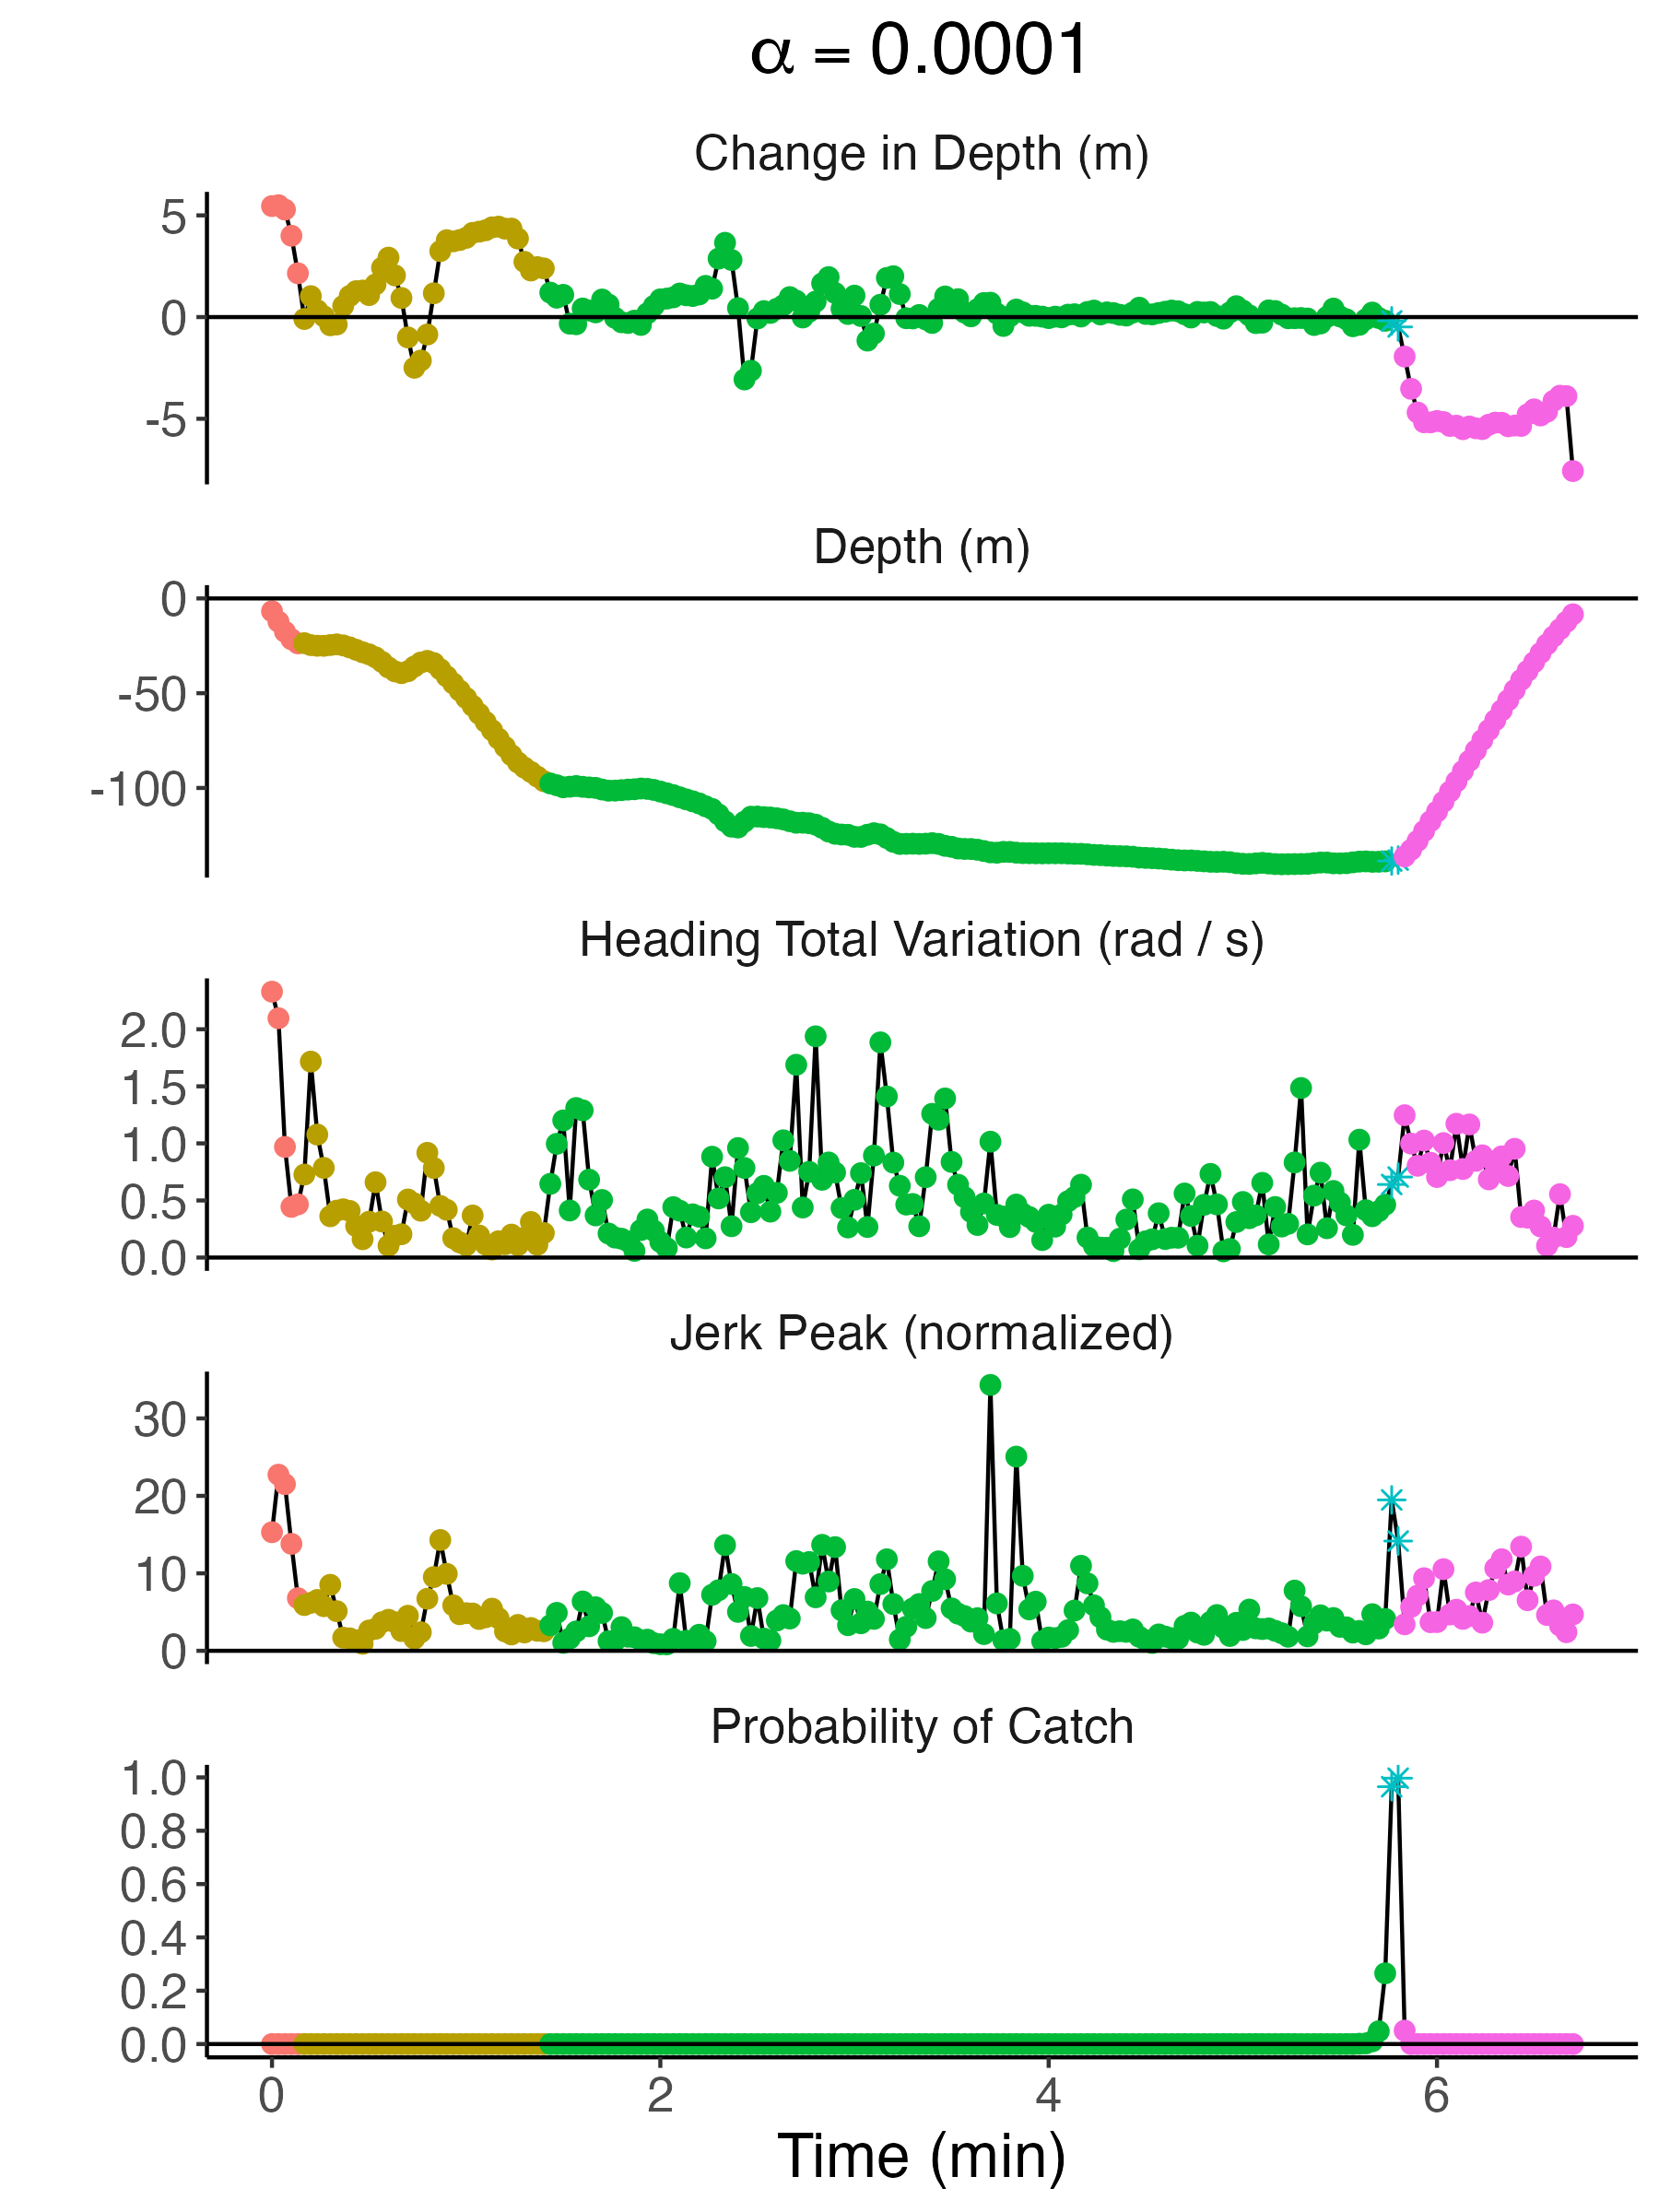
\includegraphics[height = 3.75in]{plt/profile_delt_d_htv_jp_normed_-4_4_neg_5489.png}
        %\caption{Decoded dives for PHMM with $\alpha = 0.0001$ (severely down-weighting unlabelled observations).}
    \end{subfigure}
    ~
    \begin{subfigure}[t]{0.45\textwidth}
        \centering
        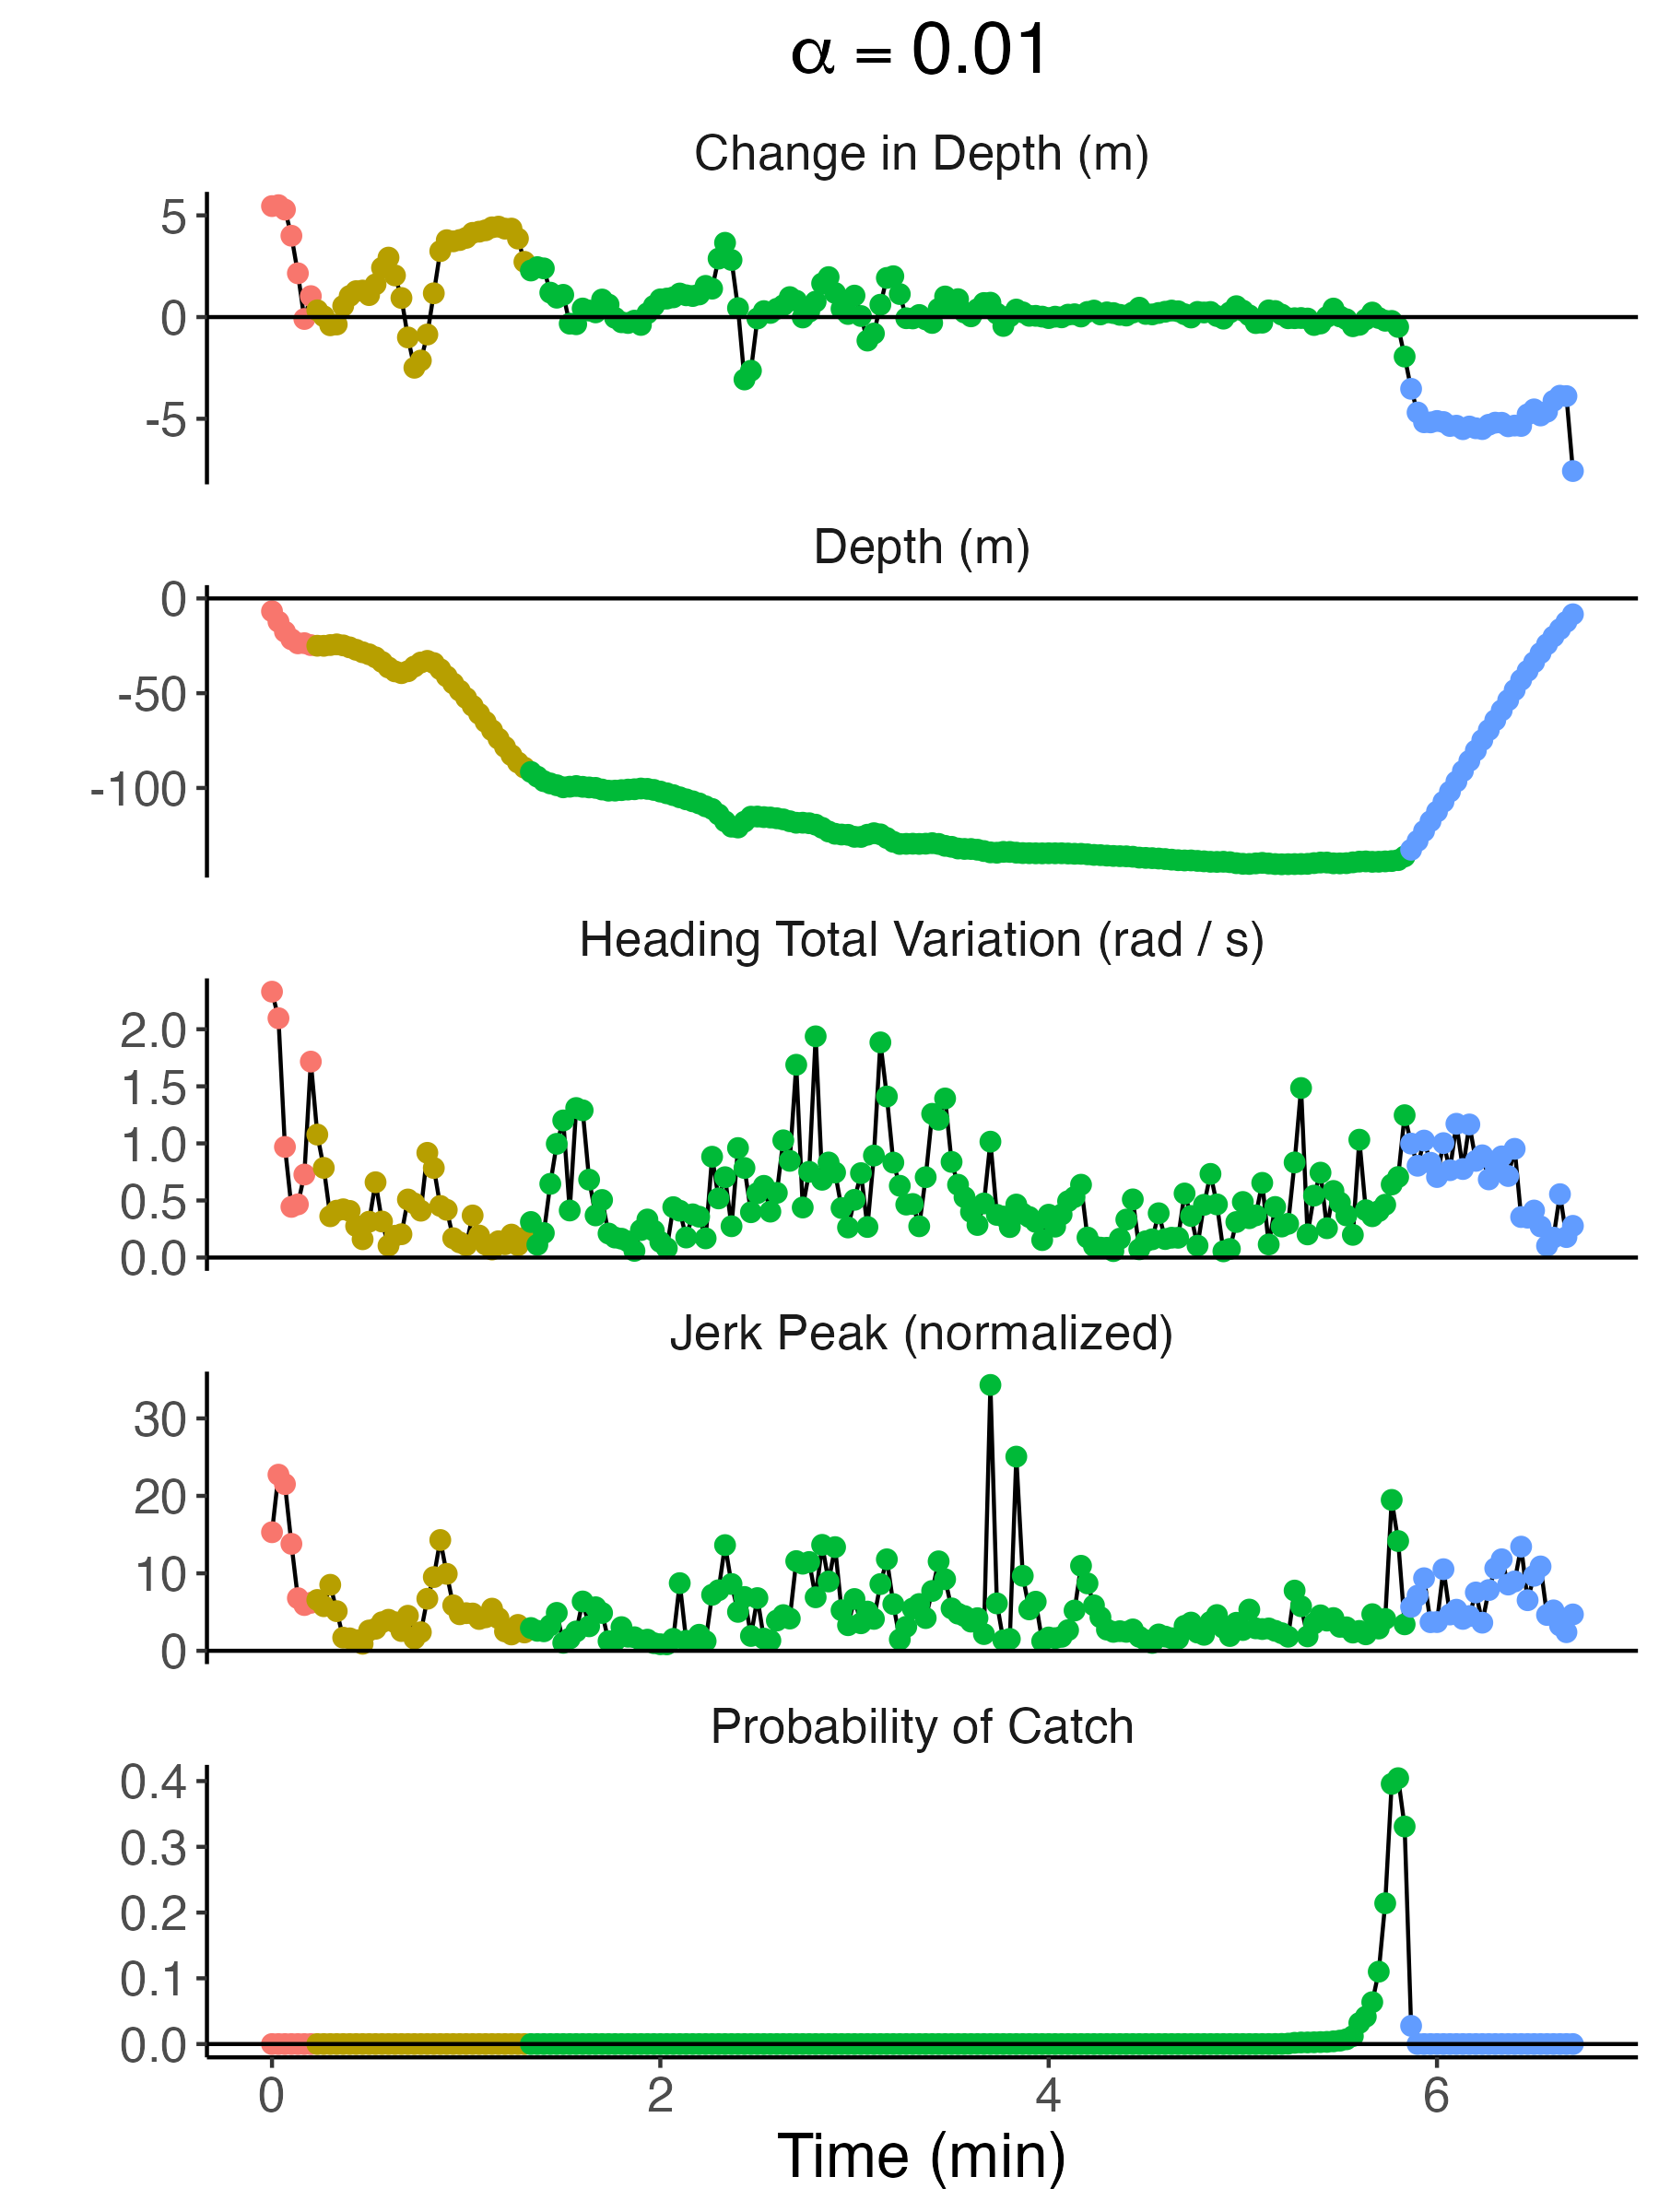
\includegraphics[height = 3.75in]{plt/profile_delt_d_htv_jp_normed_-2_4_neg_5489.png}
        %\caption{Decoded dive for PHMM with $\alpha = 0.01$ (down-weighting unlabelled observations).}
    \end{subfigure}
    \\
    \begin{subfigure}[t]{0.9\textwidth}
        \centering
        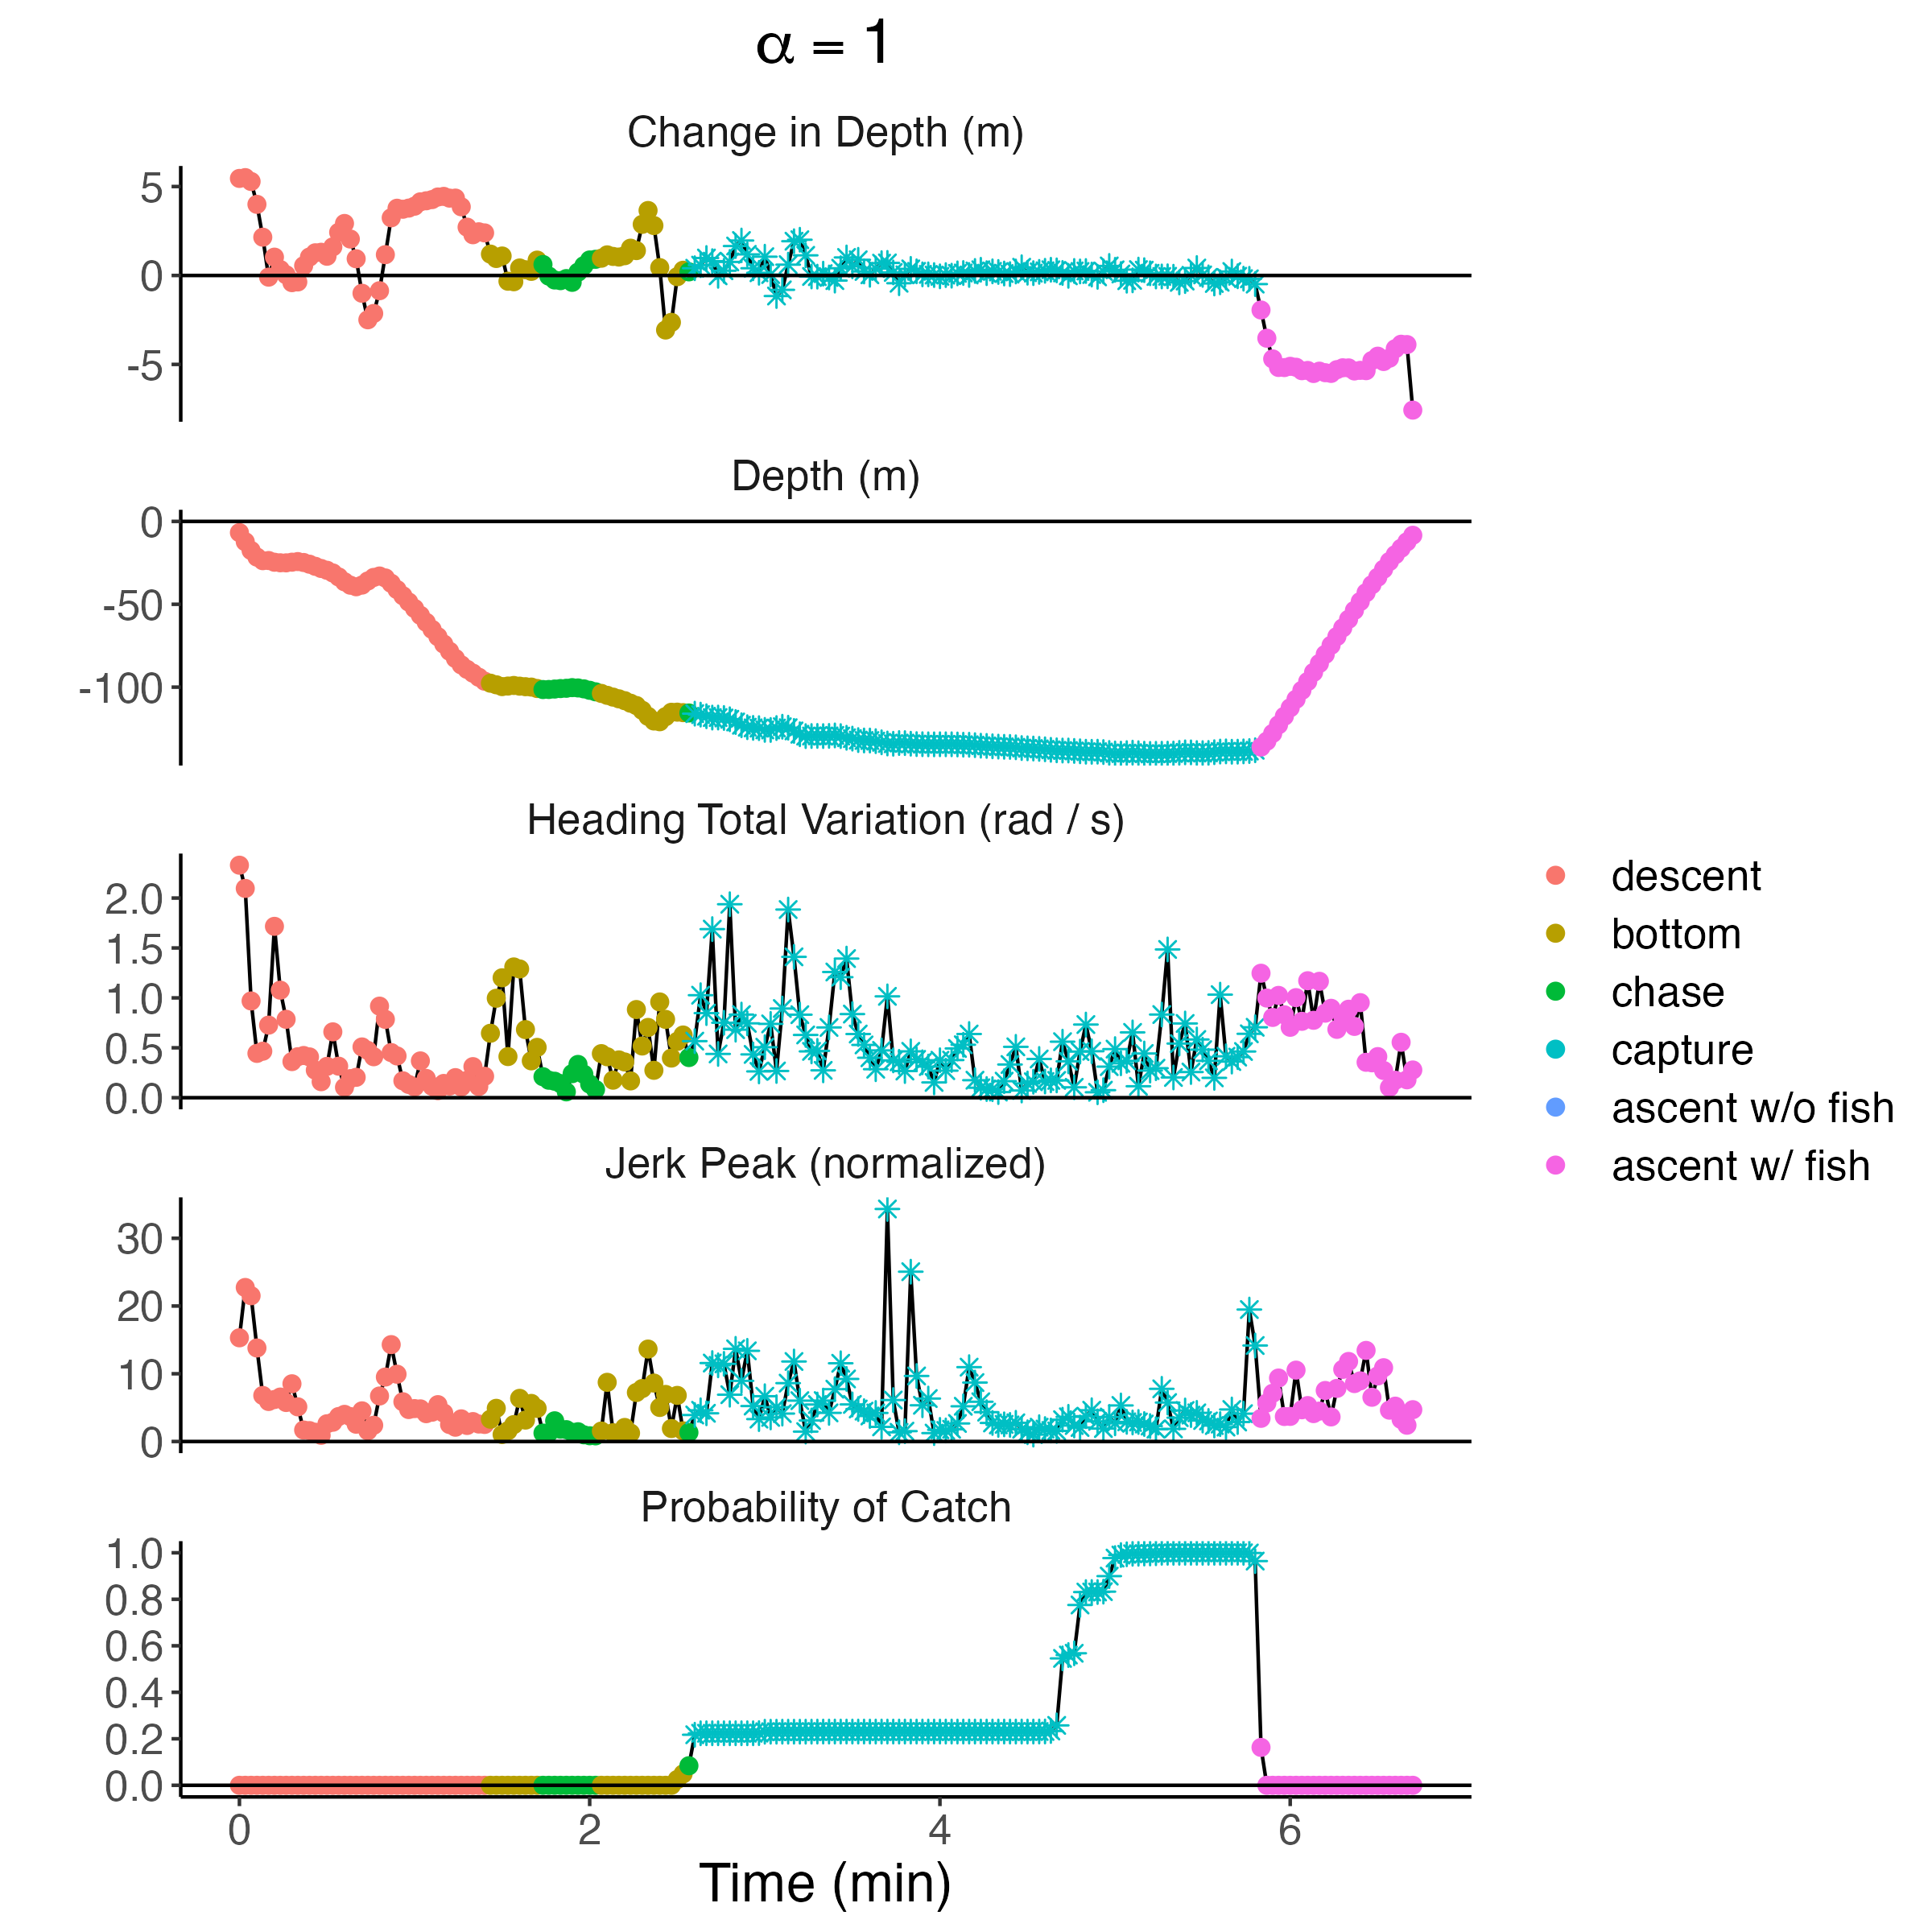
\includegraphics[height = 3.75in]{plt/profile_delt_d_htv_jp_normed_0_4_neg_5489.png}
        %\caption{Decoded dives for PHMM with $\alpha = 1$ (the ``natural" weighting).}
    \end{subfigure}
    \caption{Dive profiles, observations, and the decoded probability that each window is the ``capture" state for a selected dive with no foraging in case study 2. PHMMs with $\alpha = 0.0001$ (top left), $\alpha = 0.01$ (top right) and $\alpha = 1$ (bottom) are shown. Each subplot displays change in depth (top panel), raw depth (second panel), heading total variation (third panel), normalized jerk peak (fourth panel), and probability of ``capture" (bottom panel). Observations are coloured according to the most-likely sequence of hidden states as determined by the Viterbi algorithm. The estimated probability of successful foraging, $\bbP(X_{s,T_s} \in \{4,6\} \mid \bfY_s = \bfy_s)$, is 1 for $\alpha = 0.0001$, 0.414 for $\alpha = 0.01$, and 1 for $\alpha = 1$.}
    \label{fig:profiles_5489}
\end{figure}

Finally, I used the the PHMM with $\alpha = 0.01$ to estimate the total number of successful foraging dives from southern and northern resident killer whales in this data set. In particular, I fit the full model to the entire dataset, including labels, and then ran the forward-backward algorithm on all unlabelled dives to estimate the probability that each unlabelled dive was a successful foraging dive, $\bbP(X_{s,T_s} \in \{4,6\} \mid \bfY_s = \bfy_s)$ for $s = 1,\ldots,130$. Then, I labelled dive $s$ as a successful foraging dive if the estimate of this probability was above 50\%. This process resulted in 6 estimated successful foraging dives from southern resident killer whales and 37 estimated successful foraging dives from northern resident killer whales. After combining these results with those from the first case study, I found that southern resident killer whales caught an average of 1.03 fish per hour of foraging effort, while northern resident killer whales caught an average of 2.00 fish per hour of foraging effort. These results support the finding that northern resident killer whales have more foraging success compared to southern residents \citep{Tennessen:2023}. However, my sample size is small (2 southern resident killer whales and 9 northern resident killer whales). Future studies can use the methods outlined here to further investigate the differences between northern and resident killer whale foraging success.